\documentclass[mstat,12pt]{unswthesis}

\usepackage{color}
\usepackage{fancyvrb}
\newcommand{\VerbBar}{|}
\newcommand{\VERB}{\Verb[commandchars=\\\{\}]}
\DefineVerbatimEnvironment{Highlighting}{Verbatim}{commandchars=\\\{\}}
% Add ',fontsize=\small' for more characters per line
\usepackage{framed}
\definecolor{shadecolor}{RGB}{248,248,248}
\newenvironment{Shaded}{\begin{snugshade}}{\end{snugshade}}
\newcommand{\AlertTok}[1]{\textcolor[rgb]{0.94,0.16,0.16}{#1}}
\newcommand{\AnnotationTok}[1]{\textcolor[rgb]{0.56,0.35,0.01}{\textbf{\textit{#1}}}}
\newcommand{\AttributeTok}[1]{\textcolor[rgb]{0.13,0.29,0.53}{#1}}
\newcommand{\BaseNTok}[1]{\textcolor[rgb]{0.00,0.00,0.81}{#1}}
\newcommand{\BuiltInTok}[1]{#1}
\newcommand{\CharTok}[1]{\textcolor[rgb]{0.31,0.60,0.02}{#1}}
\newcommand{\CommentTok}[1]{\textcolor[rgb]{0.56,0.35,0.01}{\textit{#1}}}
\newcommand{\CommentVarTok}[1]{\textcolor[rgb]{0.56,0.35,0.01}{\textbf{\textit{#1}}}}
\newcommand{\ConstantTok}[1]{\textcolor[rgb]{0.56,0.35,0.01}{#1}}
\newcommand{\ControlFlowTok}[1]{\textcolor[rgb]{0.13,0.29,0.53}{\textbf{#1}}}
\newcommand{\DataTypeTok}[1]{\textcolor[rgb]{0.13,0.29,0.53}{#1}}
\newcommand{\DecValTok}[1]{\textcolor[rgb]{0.00,0.00,0.81}{#1}}
\newcommand{\DocumentationTok}[1]{\textcolor[rgb]{0.56,0.35,0.01}{\textbf{\textit{#1}}}}
\newcommand{\ErrorTok}[1]{\textcolor[rgb]{0.64,0.00,0.00}{\textbf{#1}}}
\newcommand{\ExtensionTok}[1]{#1}
\newcommand{\FloatTok}[1]{\textcolor[rgb]{0.00,0.00,0.81}{#1}}
\newcommand{\FunctionTok}[1]{\textcolor[rgb]{0.13,0.29,0.53}{\textbf{#1}}}
\newcommand{\ImportTok}[1]{#1}
\newcommand{\InformationTok}[1]{\textcolor[rgb]{0.56,0.35,0.01}{\textbf{\textit{#1}}}}
\newcommand{\KeywordTok}[1]{\textcolor[rgb]{0.13,0.29,0.53}{\textbf{#1}}}
\newcommand{\NormalTok}[1]{#1}
\newcommand{\OperatorTok}[1]{\textcolor[rgb]{0.81,0.36,0.00}{\textbf{#1}}}
\newcommand{\OtherTok}[1]{\textcolor[rgb]{0.56,0.35,0.01}{#1}}
\newcommand{\PreprocessorTok}[1]{\textcolor[rgb]{0.56,0.35,0.01}{\textit{#1}}}
\newcommand{\RegionMarkerTok}[1]{#1}
\newcommand{\SpecialCharTok}[1]{\textcolor[rgb]{0.81,0.36,0.00}{\textbf{#1}}}
\newcommand{\SpecialStringTok}[1]{\textcolor[rgb]{0.31,0.60,0.02}{#1}}
\newcommand{\StringTok}[1]{\textcolor[rgb]{0.31,0.60,0.02}{#1}}
\newcommand{\VariableTok}[1]{\textcolor[rgb]{0.00,0.00,0.00}{#1}}
\newcommand{\VerbatimStringTok}[1]{\textcolor[rgb]{0.31,0.60,0.02}{#1}}
\newcommand{\WarningTok}[1]{\textcolor[rgb]{0.56,0.35,0.01}{\textbf{\textit{#1}}}}


%%%%%%%%%%%%%%%%%%%%%%%%%%%%%%%%%%%%%%%%%%%%%%%%%%%%%%%%%%%%%%%%%%
% 
% OK...Now we get to some actual input.  The first part sets up
% the title etc that will appear on the front page
%
%%%%%%%%%%%%%%%%%%%%%%%%%%%%%%%%%%%%%%%%%%%%%%%%%%%%%%%%%%%%%%%%%

\title{Projet réalisé par\\[0.5cm] l'équipe 5 du groupe de TD1 \\[3cm]Rapport
de groupe des deep learners anonymes\newline  Bases de données +
Sciences des Données 2}

\authornameonly{Alban Gerschheimer, Omar Terras, Alfred Gyalay, Mia
Portes. }

\author{\Authornameonly}

\copyrightfalse
\figurespagefalse
\tablespagefalse

%%%%%%%%%%%%%%%%%%%%%%%%%%%%%%%%%%%%%%%%%%%%%%%%%%%%%%%%%%%%%%%%%
%
%  And now the document begins
%  The \beforepreface and \afterpreface commands puts the
%  contents page etc in
%
%%%%%%%%%%%%%%%%%%%%%%%%%%%%%%%%%%%%%%%%%%%%%%%%%%%%%%%%%%%%%%%%%%


\input{header.tex}

\renewcommand{\contentsname}{Table des matières}

\renewcommand{\chaptername}{Chapitre}




\begin{document}

\beforepreface

%\afterpage{\blankpage}

% plagiarism

\prefacesection{Déclaration de non plagiat}

\vskip 2pc \noindent Nous déclarons que ce rapport est le fruit de notre seul travail, à part lorsque cela est indiqué  explicitement. 

\vskip 2pc  \noindent Nous acceptons que la personne évaluant ce rapport puisse, pour les besoins de cette évaluation:
\begin{itemize}
\item la reproduire et en fournir une copie à un autre membre de l'université; et/ou,
\item en communiquer une copie à un service en ligne de détection de plagiat (qui pourra en retenir une copie pour les besoins d'évaluation future).
\end{itemize}

\vskip 2pc \noindent Nous certifions que nous avons lu et compris les règles ci-dessus.\vspace{24pt}

\vskip 2pc \noindent En signant cette déclaration, nous acceptons ce qui précède.
\vskip 2pc \noindent
%%Signature: \rule{7cm}{0.25pt} \hfill Date: \rule{4cm}{0.25pt} \\[1cm]
%%Signature: \rule{7cm}{0.25pt} \hfill Date: \rule{4cm}{0.25pt} \\[1cm]
%%Signature: \rule{7cm}{0.25pt} \hfill Date: \rule{4cm}{0.25pt} \\[1cm]
%%Signature: \rule{7cm}{0.25pt} \hfill Date: \rule{4cm}{0.25pt} \\[1cm]
%%\vskip 1pc
Signature : Alban Gerschheimer \hfill Date: 04/05/2025\\[1cm]
Signature : Omar Terras \hfill Date: 04/05/2025 \\[1cm]
Signature : Alfred Gyalay \hfill Date: 04/05/2025\\[1cm]
Signature : Mia Portes \hfill Date: 04/05/2025\\[1cm]

%\textcolor{red}{Mettre à jour la date.}

{\bigskip\bigskip\bigskip\noindent} \today
%\afterpage{\blankpage}

% Acknowledgements are optional


\prefacesection{Remerciements}


{\bigskip}Nous tenons à remercier nos enseignantes, Mme Sandra Bringay
et Mme Marine Demangeot, pour leur soutien et leurs conseils précieux
tout au long de ce projet.\\[1cm] Nous remercions également les membres
de ce groupe pour leur sérieux et leur implication tout au long de sa
réalisation.\\[1cm] 

{\bigskip\bigskip\bigskip\noindent} \today

%\afterpage{\blankpage}

% Abstract

\prefacesection{Résumé}

L'image ci-dessous vous donne quelques conseils pour rédiger un bon
résumé.\newline 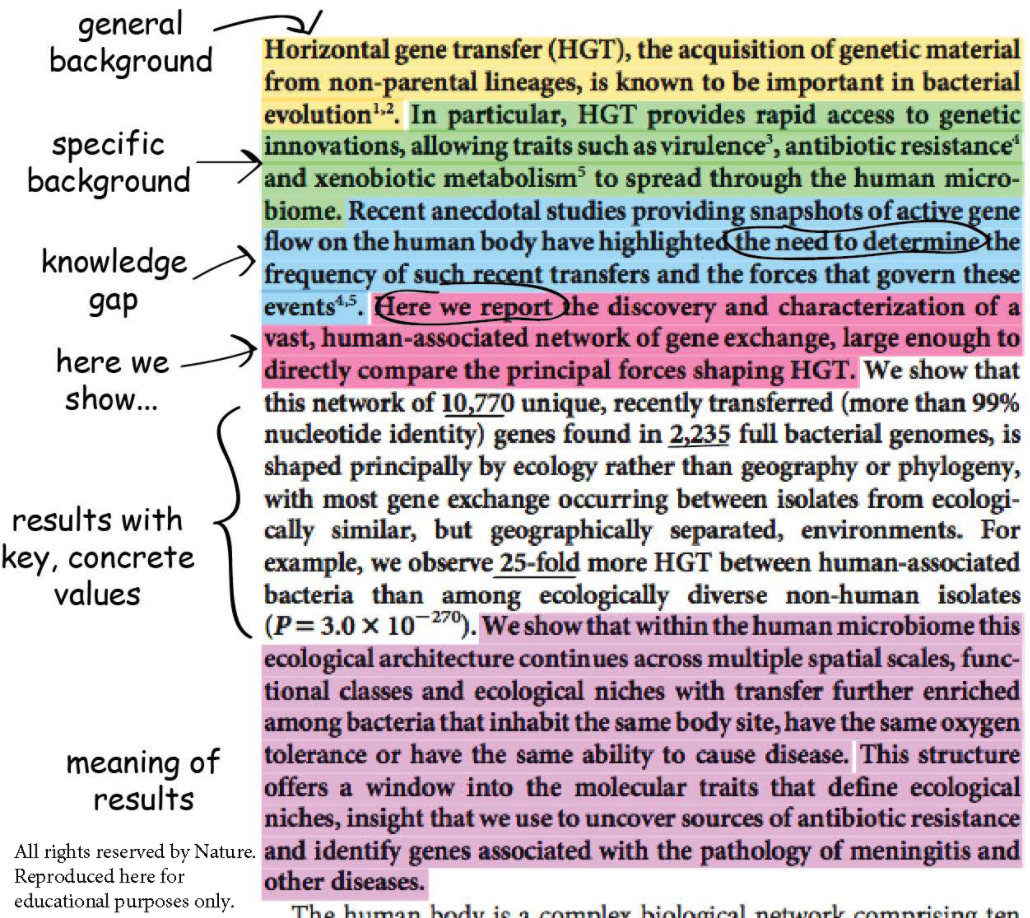
\includegraphics[width=10cm,height=10cm]{scdon2-UPV-report-template_files/good-abstract.png}

%\afterpage{\blankpage}


\afterpreface





%%%%%%%%%%%%%%%%%%%%%%%%%%%%%%%%%%%%%%%%%%%%%%%%%%%%%%%%%%%%%%%%%%
%
% Now we can start on the first chapter
% Within chapters we have sections, subsections and so forth
%
%%%%%%%%%%%%%%%%%%%%%%%%%%%%%%%%%%%%%%%%%%%%%%%%%%%%%%%%%%%%%%%%%%



%%%%%%%%%%%%%%%%%%%%%%%%%%%%%%%%%%%%%

%\afterpage{\blankpage}


\chapter{Introduction}\label{introduction}

\section{Introduction}\label{introduction-1}

La biodiversité marine est aujourd'hui soumise à de nombreuses pressions
humaines, notamment liées aux activités portuaires et aux installations
offshore. Les ports concentrent une forte activité maritime, logistique
et industrielle, tandis que les infrastructures offshore modifient
également les espaces marins. Il est donc pertinent de se poser la
question suivante:

\bigskip

\begin{center}

\textbf{Dans quelle mesure la proximité des ports maritimes et des infrastructures offshore influence-t-elle la distribution spatiale des observations de biodiversité marine en Europe ?
}

\end{center}
\medskip

\justifying

Cette problématique s'appuie sur plusieurs sources de données réelles :
des occurrences d'espèces marines issues de GBIF(mettre lien), des
données géographiques sur les ports maritimes(mettre lien), ainsi que
des données sur des infrastructures offshore(mettre lien).

\medskip

L'objectif est de construire une base de données relationnelle
permettant de croiser ces informations, puis de réaliser des requêtes
SQL afin de dégager des tendances exploitables dans le cadre du cours de
Sciences des données 2.

\medskip

Le cadre du projet demande justement d'utiliser plusieurs sources
réelles, de les intégrer dans une base relationnelle, puis de les
interroger pour produire des tableaux et analyses.

\medskip

Nous avons retenu ces jeux de données car ils permettent de croiser une
information biologique, à savoir les occurrences d'espèces marines, avec
des informations spatiales décrivant certaines pressions anthropiques.
Ce croisement est cohérent avec notre problématique, qui porte sur
l'influence potentielle des ports et des infrastructures offshore sur la
distribution observée de la biodiversité marine.

\section{Responsabilités et composition de
l'équipe}\label{responsabilituxe9s-et-composition-de-luxe9quipe}

Dans notre équipe, les taches ont été réparties de la manière suivante:

\medskip

Alban Gerschheimer: Étudiant n°XXXX, Resp. de l'import de données et des
requêtes SQL.

Omar Terras: Étudiant n°XXXX, Resp.

Alfred Gyalay: Étudiant n°XXXX, Resp. du code R.

Mia Portes : Étudiant n°22406297, Resp. du rapport.

\chapter{Base de données}\label{base-de-donnuxe9es}

\section{Provenance des données}\label{provenance-des-donnuxe9es}

Nous avons décidé de choisir des datas selon certains critères afin de
garder une cohérence lors de cette recherche.

Les critères appliqués sont les suivants :

\begin{itemize}
\item zone : \textbf{Europe maritime}
\item période : \textbf{2010–2026}
\item espèces : \textbf{uniquement 3 grands groupes}
\item observations : \textbf{présentes uniquement}
\item coordonnées : \textbf{obligatoires}
\item problèmes spatiaux : \textbf{exclusion des observations avec un problème géospatial}
\item profondeur : \textbf{plus petit ou égal à 0}
\end{itemize}

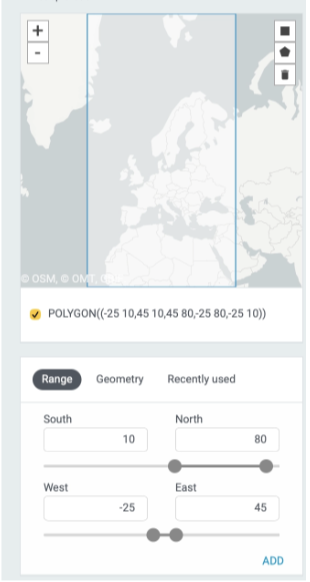
\includegraphics[width=4cm,height=\textheight,keepaspectratio]{scdon2-UPV-report-template_files/img1.png}
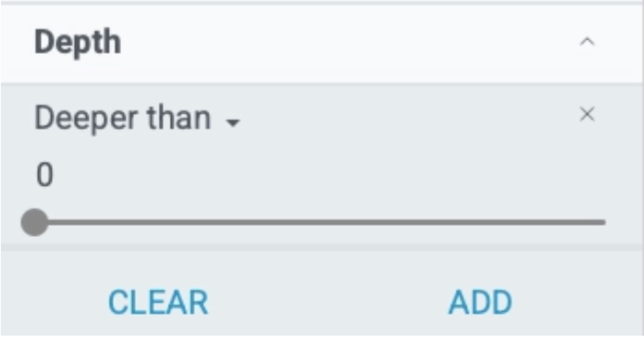
\includegraphics[width=\linewidth,height=3cm,keepaspectratio]{scdon2-UPV-report-template_files/img2.png}

Chaque observation d'espèce sera localisée à l'aide de ses coordonnées
géographiques, puis comparée à la position des ports et des
infrastructures offshore les plus proches. L'idée est que plus une
observation est proche d'un port ou d'une infrastructure, plus elle est
susceptible d'être soumise à une pression humaine potentielle. À
l'inverse, les observations éloignées seront considérées comme situées
dans des zones moins directement influencées.

\bigskip

\section{Distance entre une observation et un
port/plateforme}\label{distance-entre-une-observation-et-un-portplateforme}

Pour chaque observation, nous calculerons la distance avec les ports
maritimes présents dans notre base.\newline Si une observation a pour
coordonnées (lat\_o, lon\_o) et un port (lat\_p, lon\_p), alors on
calcule une distance géographique entre les deux points à l'aide de la
formule suivante:

\[
d_{port}(o,p)=\sqrt{(lat_o - lat_p)^2 + (lon_o - lon_p)^2}
\]

Cette formule donne une distance euclidienne simplifiée entre une
observation o et un port p.

\bigskip

Ensuite, pour chaque observation, on garde seulement la distance au port
\textbf{le plus proche}. On applique la même logique aux infrastructures
offshore. Pour une observation o et une infrastructure i, la distance
peut être notée :

\[
d_{infra}(o,i)=\sqrt{(lat_o - lat_i)^2 + (lon_o - lon_i)^2}
\] Puis on retient la \textbf{distance minimale}.

\section{Construction de classes de
distance}\label{construction-de-classes-de-distance}

Afin de rendre l'analyse plus lisible, les distances minimales calculées
entre chaque observation et le port ou l'infrastructure offshore les
plus proches n'ont pas seulement été conservées sous forme numérique.
Elles ont aussi été transformées en classes de proximité, enregistrées
dans les variables classe\_distance\_port et classe\_distance\_infra.

Dans notre codage, une valeur élevée correspond à une observation plus
proche, tandis qu'une valeur faible correspond à une observation plus
éloignée. Ce regroupement permet de comparer plus facilement la
distribution des observations, le nombre d'espèces distinctes et la
répartition des groupes taxonomiques selon le niveau de proximité aux
ports et aux infrastructures offshore. Son echelle est de 1 à 10.

\section{Descriptif des tables}\label{descriptif-des-tables}

\textbf{REMPLIR LE NOMBRE DE COLONNES ET DE LIGNES}

\begin{longtable}[]{@{}
  >{\centering\arraybackslash}p{(\linewidth - 6\tabcolsep) * \real{0.1604}}
  >{\centering\arraybackslash}p{(\linewidth - 6\tabcolsep) * \real{0.0755}}
  >{\centering\arraybackslash}p{(\linewidth - 6\tabcolsep) * \real{0.3585}}
  >{\centering\arraybackslash}p{(\linewidth - 6\tabcolsep) * \real{0.4057}}@{}}
\caption{Espece (nombre de lignes \(\times\) nombre de
colonnes)}\tabularnewline
\toprule\noalign{}
\begin{minipage}[b]{\linewidth}\centering
Nom colonne
\end{minipage} & \begin{minipage}[b]{\linewidth}\centering
Type
\end{minipage} & \begin{minipage}[b]{\linewidth}\centering
Signification
\end{minipage} & \begin{minipage}[b]{\linewidth}\centering
Caractéristique
\end{minipage} \\
\midrule\noalign{}
\endfirsthead
\toprule\noalign{}
\begin{minipage}[b]{\linewidth}\centering
Nom colonne
\end{minipage} & \begin{minipage}[b]{\linewidth}\centering
Type
\end{minipage} & \begin{minipage}[b]{\linewidth}\centering
Signification
\end{minipage} & \begin{minipage}[b]{\linewidth}\centering
Caractéristique
\end{minipage} \\
\midrule\noalign{}
\endhead
\bottomrule\noalign{}
\endlastfoot
id\_espece & Entier & Identifiant unique de l'espèce & Clé primaire,
unique, non nul \\
scientific\_name & Texte & Nom scientifique complet de l'espèce & Non
unique, non nul \\
phylum & Texte & Embranchement taxonomique & Non unique, peut contenir
des répétitions \\
classe & Texte & Classe taxonomique de l'espèce & Non unique \\
ordre & Texte & Ordre taxonomique de l'espèce & Non unique \\
famille & Texte & Famille taxonomique de l'espèce & Non unique \\
genre & Texte & Genre taxonomique de l'espèce & Non unique \\
nom\_espece & Texte & Nom spécifique de l'espèce & Non unique, parfois
valeur manquante \\
\end{longtable}

\begin{longtable}[]{@{}
  >{\centering\arraybackslash}p{(\linewidth - 6\tabcolsep) * \real{0.1575}}
  >{\centering\arraybackslash}p{(\linewidth - 6\tabcolsep) * \real{0.1024}}
  >{\centering\arraybackslash}p{(\linewidth - 6\tabcolsep) * \real{0.3543}}
  >{\centering\arraybackslash}p{(\linewidth - 6\tabcolsep) * \real{0.3858}}@{}}
\caption{Observation (nombre de lignes \(\times\) nombre de
colonnes)}\tabularnewline
\toprule\noalign{}
\begin{minipage}[b]{\linewidth}\centering
Nom colonne
\end{minipage} & \begin{minipage}[b]{\linewidth}\centering
Type
\end{minipage} & \begin{minipage}[b]{\linewidth}\centering
Signification
\end{minipage} & \begin{minipage}[b]{\linewidth}\centering
Caractéristique
\end{minipage} \\
\midrule\noalign{}
\endfirsthead
\toprule\noalign{}
\begin{minipage}[b]{\linewidth}\centering
Nom colonne
\end{minipage} & \begin{minipage}[b]{\linewidth}\centering
Type
\end{minipage} & \begin{minipage}[b]{\linewidth}\centering
Signification
\end{minipage} & \begin{minipage}[b]{\linewidth}\centering
Caractéristique
\end{minipage} \\
\midrule\noalign{}
\endhead
\bottomrule\noalign{}
\endlastfoot
id\_observation & Entier long & Identifiant unique de l'observation GBIF
& Clé primaire, unique, non nul \\
id\_espece & Entier & Identifiant de l'espèce observée & Clé étrangère
vers ESPECE, non nul \\
annee & Entier & Année de l'observation & Non unique, filtrée entre 2010
et 2026 \\
latitude & Décimal & Latitude de l'observation & Non nulle après
nettoyage \\
longitude & Décimal & Longitude de l'observation & Non nulle après
nettoyage \\
profondeur & Décimal & Profondeur de l'observation & Peut contenir des
valeurs nulles \\
country\_code & Texte court & Code du pays de l'observation & Non
unique \\
basis\_of\_record & Texte & Type d'enregistrement de l'observation & Non
unique \\
occurrence\_status & Texte & Statut de présence de l'espèce observée &
Valeur conservée : present \\
dataset\_key & Texte & Identifiant du jeu de données source & Non
unique \\
\end{longtable}

\begin{longtable}[]{@{}
  >{\centering\arraybackslash}p{(\linewidth - 6\tabcolsep) * \real{0.1527}}
  >{\centering\arraybackslash}p{(\linewidth - 6\tabcolsep) * \real{0.1679}}
  >{\centering\arraybackslash}p{(\linewidth - 6\tabcolsep) * \real{0.2977}}
  >{\centering\arraybackslash}p{(\linewidth - 6\tabcolsep) * \real{0.3817}}@{}}
\caption{Port (nombre de lignes \(\times\) nombre de
colonnes)}\tabularnewline
\toprule\noalign{}
\begin{minipage}[b]{\linewidth}\centering
Nom colonne
\end{minipage} & \begin{minipage}[b]{\linewidth}\centering
Type
\end{minipage} & \begin{minipage}[b]{\linewidth}\centering
Signification
\end{minipage} & \begin{minipage}[b]{\linewidth}\centering
Caractéristique
\end{minipage} \\
\midrule\noalign{}
\endfirsthead
\toprule\noalign{}
\begin{minipage}[b]{\linewidth}\centering
Nom colonne
\end{minipage} & \begin{minipage}[b]{\linewidth}\centering
Type
\end{minipage} & \begin{minipage}[b]{\linewidth}\centering
Signification
\end{minipage} & \begin{minipage}[b]{\linewidth}\centering
Caractéristique
\end{minipage} \\
\midrule\noalign{}
\endhead
\bottomrule\noalign{}
\endlastfoot
id\_port & Entier ou texte court & Identifiant unique du port & Clé
primaire, unique, non nul \\
code\_port & Texte court & Code du port lorsqu'il existe & Peut être
unique selon la source, parfois nul \\
nom\_port & Texte & Nom du port maritime & Non unique dans l'absolu, non
nul si conservé \\
activite\_principale & Texte & Activité principale ou type de port &
Peut contenir des répétitions, peut être nulle \\
latitude\_port & Décimal & Latitude du port & Non nulle après
nettoyage \\
longitude\_port & Décimal & Longitude du port & Non nulle après
nettoyage \\
\end{longtable}

\begin{longtable}[]{@{}
  >{\centering\arraybackslash}p{(\linewidth - 6\tabcolsep) * \real{0.1298}}
  >{\centering\arraybackslash}p{(\linewidth - 6\tabcolsep) * \real{0.1679}}
  >{\centering\arraybackslash}p{(\linewidth - 6\tabcolsep) * \real{0.3740}}
  >{\centering\arraybackslash}p{(\linewidth - 6\tabcolsep) * \real{0.3282}}@{}}
\caption{Infrastructure (nombre de lignes \(\times\) nombre de
colonnes)}\tabularnewline
\toprule\noalign{}
\begin{minipage}[b]{\linewidth}\centering
Nom colonne
\end{minipage} & \begin{minipage}[b]{\linewidth}\centering
Type
\end{minipage} & \begin{minipage}[b]{\linewidth}\centering
Signification
\end{minipage} & \begin{minipage}[b]{\linewidth}\centering
Caractéristique
\end{minipage} \\
\midrule\noalign{}
\endfirsthead
\toprule\noalign{}
\begin{minipage}[b]{\linewidth}\centering
Nom colonne
\end{minipage} & \begin{minipage}[b]{\linewidth}\centering
Type
\end{minipage} & \begin{minipage}[b]{\linewidth}\centering
Signification
\end{minipage} & \begin{minipage}[b]{\linewidth}\centering
Caractéristique
\end{minipage} \\
\midrule\noalign{}
\endhead
\bottomrule\noalign{}
\endlastfoot
id\_infra & Entier ou texte court & Identifiant unique de
l'infrastructure offshore & Clé primaire, unique, non nul \\
type\_infra & Texte & Type d'infrastructure offshore & Non unique \\
label & Texte & Libellé ou nom de l'infrastructure & Non unique, peut
être descriptif \\
date\_releve & Date ou texte & Date du relevé ou de mise à jour &
\textbf{MANQUANT} \\
latitude\_infra & Décimal & Latitude de l'infrastructure & Non nulle
après nettoyage \\
longitude\_infra & Décimal & Longitude de l'infrastructure & Non nulle
après nettoyage \\
\end{longtable}

\begin{longtable}[]{@{}
  >{\centering\arraybackslash}p{(\linewidth - 6\tabcolsep) * \real{0.1631}}
  >{\centering\arraybackslash}p{(\linewidth - 6\tabcolsep) * \real{0.1560}}
  >{\centering\arraybackslash}p{(\linewidth - 6\tabcolsep) * \real{0.3191}}
  >{\centering\arraybackslash}p{(\linewidth - 6\tabcolsep) * \real{0.3617}}@{}}
\caption{Localiser X (nombre de lignes \(\times\) nombre de
colonnes)}\tabularnewline
\toprule\noalign{}
\begin{minipage}[b]{\linewidth}\centering
Nom colonne
\end{minipage} & \begin{minipage}[b]{\linewidth}\centering
Type
\end{minipage} & \begin{minipage}[b]{\linewidth}\centering
Signification
\end{minipage} & \begin{minipage}[b]{\linewidth}\centering
Caractéristique
\end{minipage} \\
\midrule\noalign{}
\endfirsthead
\toprule\noalign{}
\begin{minipage}[b]{\linewidth}\centering
Nom colonne
\end{minipage} & \begin{minipage}[b]{\linewidth}\centering
Type
\end{minipage} & \begin{minipage}[b]{\linewidth}\centering
Signification
\end{minipage} & \begin{minipage}[b]{\linewidth}\centering
Caractéristique
\end{minipage} \\
\midrule\noalign{}
\endhead
\bottomrule\noalign{}
\endlastfoot
id\_observation & Entier long & Identifiant de l'observation étudiée &
Clé étrangère vers OBSERVATION \\
id\_X & Entier ou texte court & Identifiant de X lié à l'observation &
Clé étrangère vers X \\
distance\_X & Décimal & Distance calculée entre l'observation et X & Non
négative \\
categorie\_distance\_X & Texte & Classe de distance entre l'observation
et X & Exemples : très\_proche, proche, moyenne, éloignée \\
\end{longtable}

\section{Modèle MCD:}\label{moduxe8le-mcd}

\begin{figure}
\centering
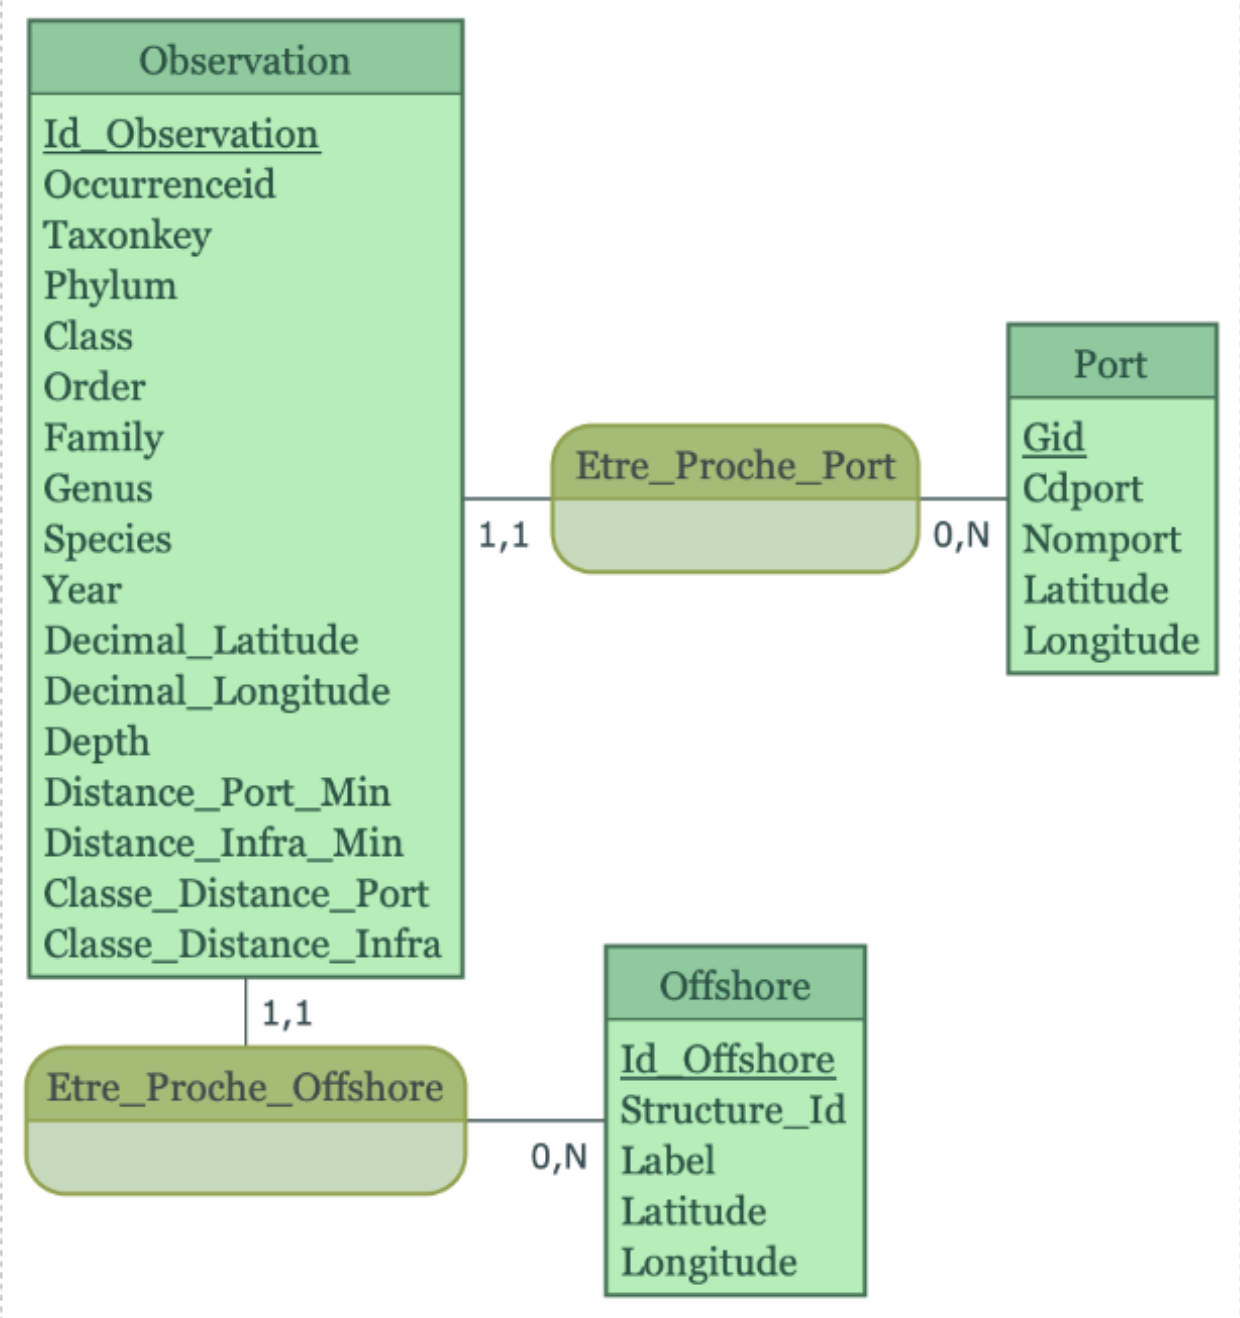
\includegraphics[width=7cm,height=\textheight,keepaspectratio]{scdon2-UPV-report-template_files/MCD.png}
\caption{Relations.}\label{uml}
\end{figure}

\section{Modèle MOD:}\label{moduxe8le-mod}

OBSERVATION(id\_observation, occurrenceid, taxonkey, phylum, class,
order, family, genus, species, year, decimalLatitude, decimalLongitude,
depth, distance\_port\_min, distance\_infra\_min,
classe\_distance\_port, classe\_distance\_infra, gid\_port\_proche\#,
id\_offshore\_proche\#)

PORT(gid, cdport, nomport, latitude, longitude)

OFFSHORE(id\_offshore, structure\_id, label, latitude, longitude)

\begin{figure}
\centering
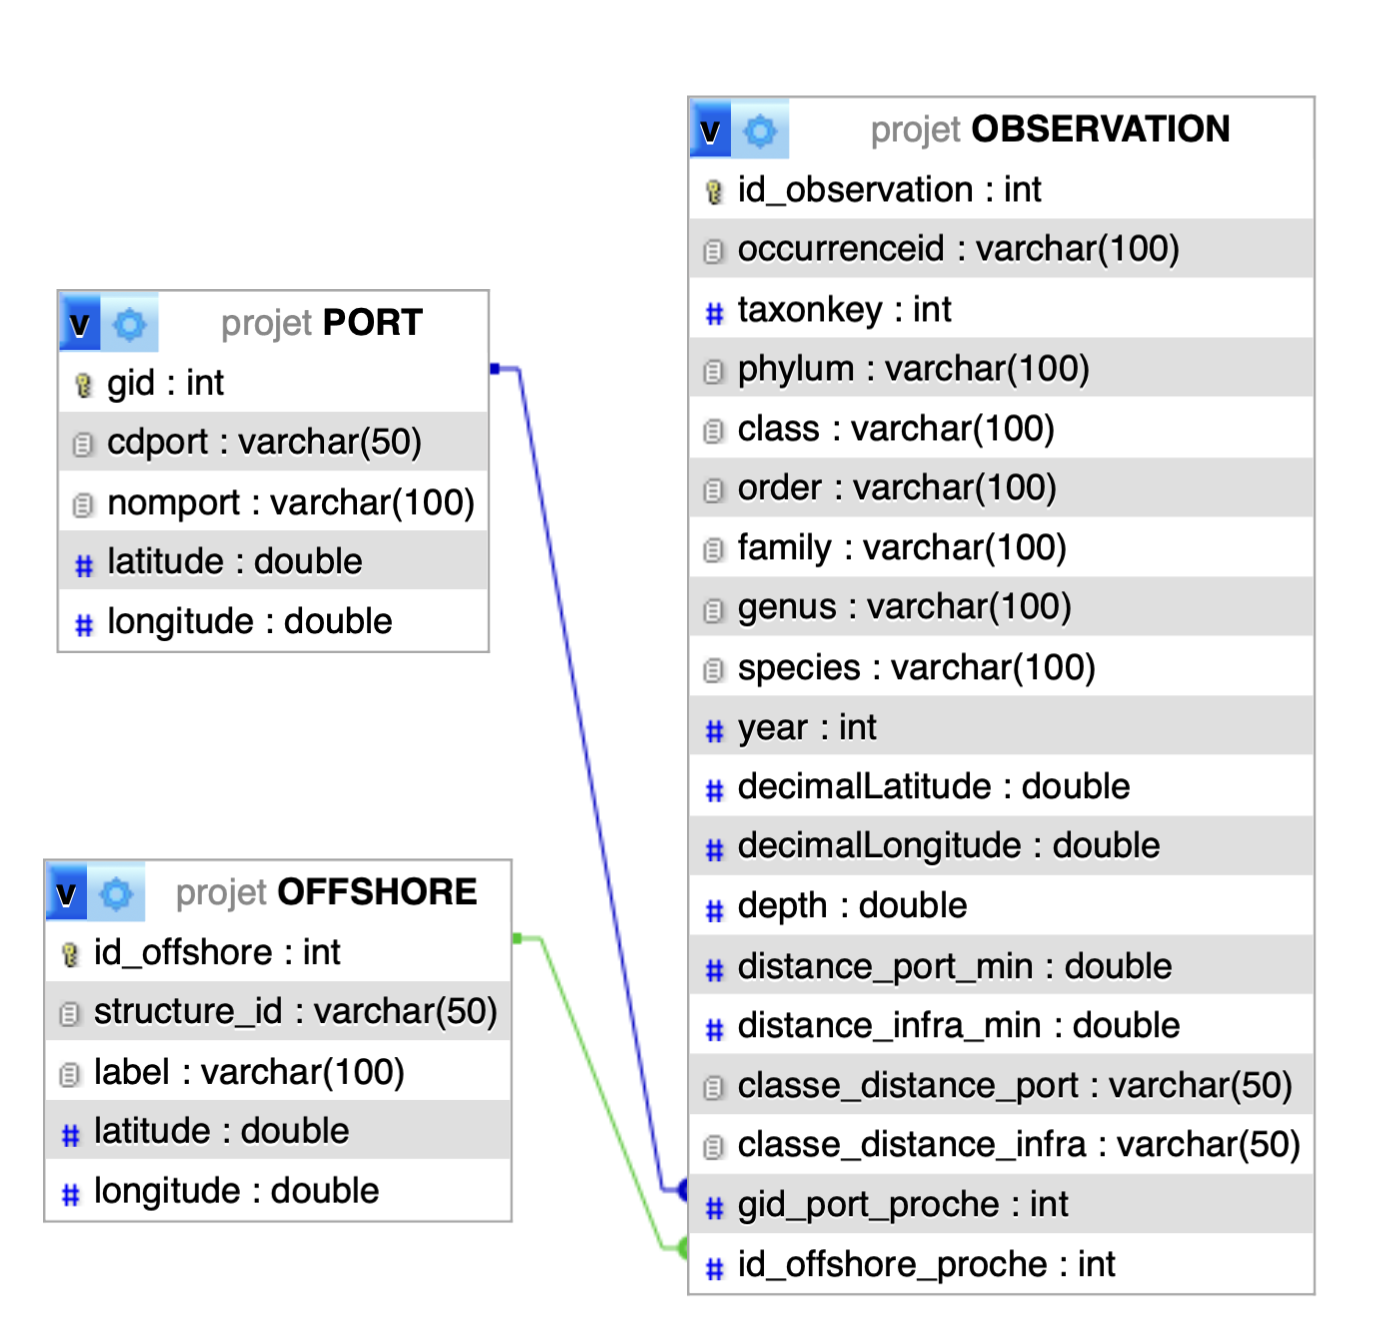
\includegraphics[width=8cm,height=\textheight,keepaspectratio]{scdon2-UPV-report-template_files/MOD.png}
\caption{Tables.}\label{uml2}
\end{figure}

\section{Importation et préparation des
données}\label{importation-et-pruxe9paration-des-donnuxe9es}

\subsection{Création de la base de
données}\label{cruxe9ation-de-la-base-de-donnuxe9es}

Dans cette partie nous allons utiliser DBpro et Python ainsi que la
bibliothèque pandas. Avant l'importation des données, une phase de
préparation a été réalisée afin de garantir la qualité et la cohérence
des informations exploitées. Une nouvelle base de données nommée
\textbf{base\_maritime\_europeenne} a été créée.

\begin{figure}
\centering

\includegraphics[width=7cm,height=\textheight,keepaspectratio]{scdon2-UPV-report-template_files/base.png}
\caption{Base.}\label{uml}
\end{figure}

\subsection{Importation et organisation des
tables}\label{importation-et-organisation-des-tables}

Les différentes tables ont ensuite été importées dans la base de
données.

\begin{figure}
\centering
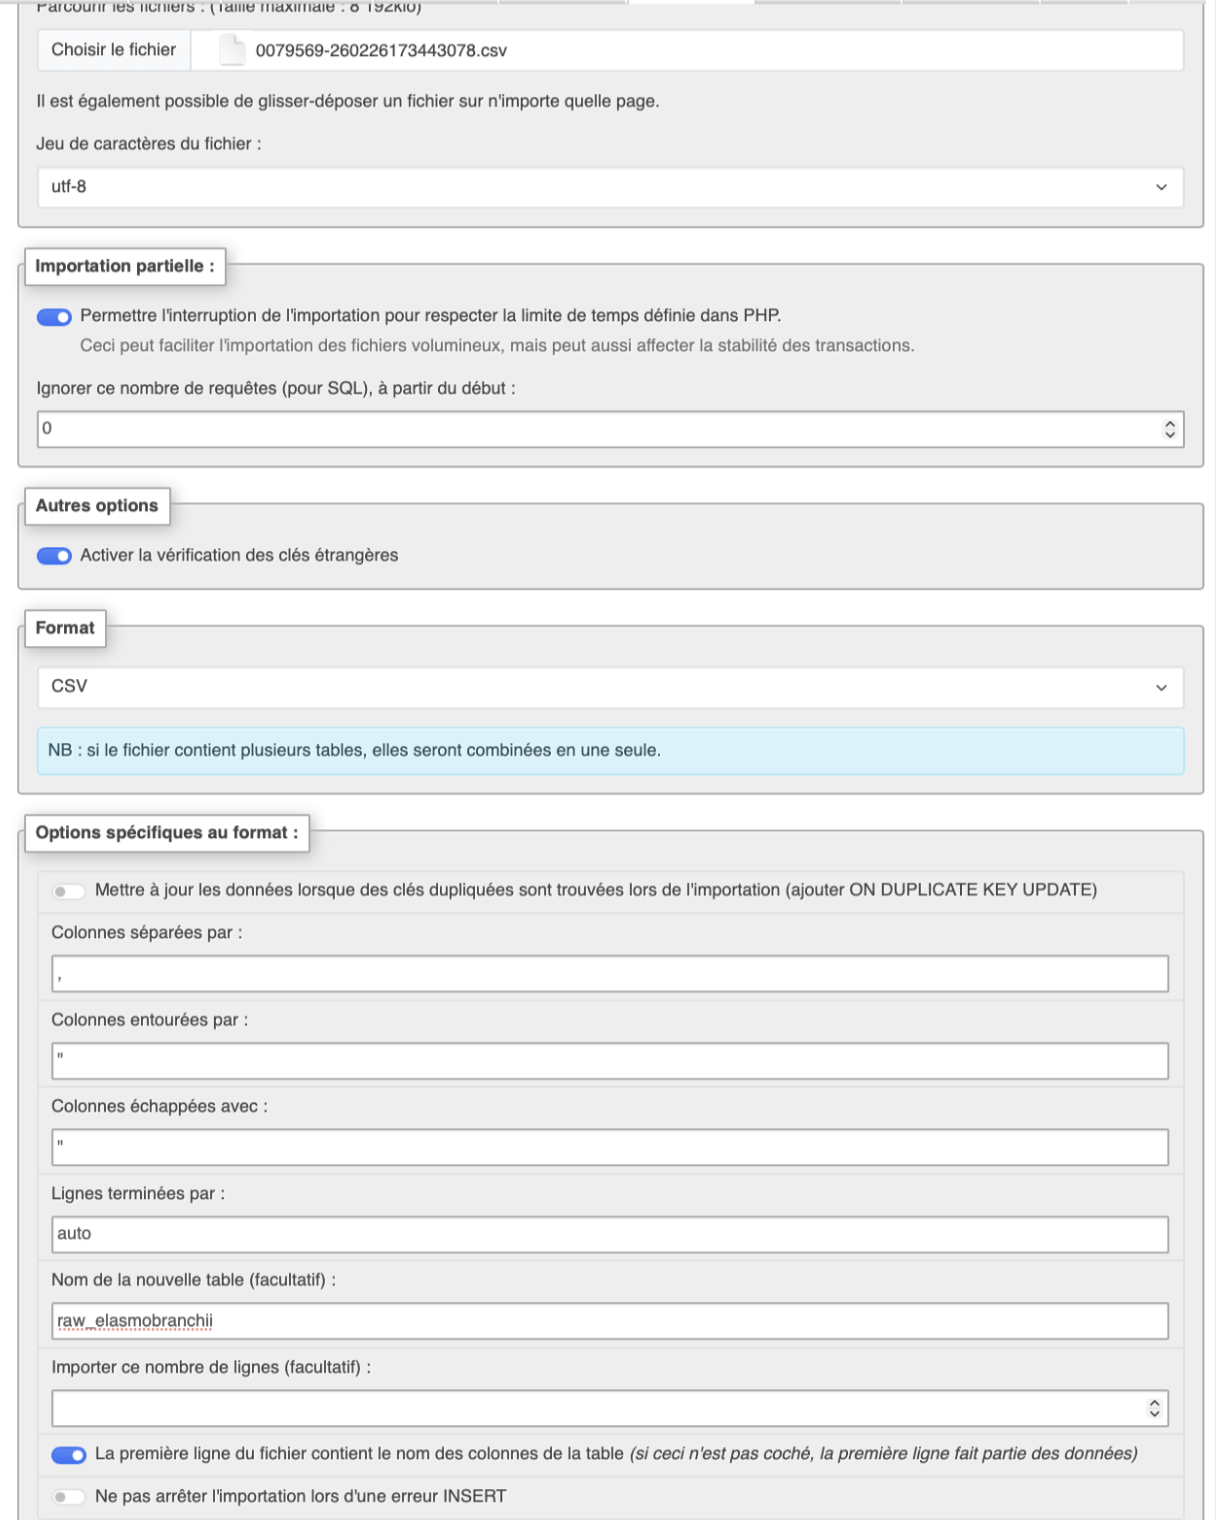
\includegraphics[width=5cm,height=\textheight,keepaspectratio]{scdon2-UPV-report-template_files/import.png}
\caption{Importation.}\label{uml}
\end{figure}

Après importation, les tables ont été renommées comme suit :

\begin{itemize}
\tightlist
\item
  elasmobranchii\_europe
\item
  cnidaria\_europe
\item
  malacostraca\_europe
\item
  port\_maritime\_eur
\item
  offshore\_europe
\end{itemize}

\subsection{Création des clés
primaires}\label{cruxe9ation-des-cluxe9s-primaires}

Certaines tables ne possédaient pas de clé primaire fiable et
contenaient des doublons. Afin d'assurer l'intégrité des données, des
identifiants techniques auto-incrémentés ont été ajoutés.

Exemple :

\begin{Shaded}
\begin{Highlighting}[]
\KeywordTok{ALTER} \KeywordTok{TABLE}\NormalTok{ cnidaria\_europe}
\KeywordTok{ADD} \KeywordTok{COLUMN}\NormalTok{ id\_obs }\DataTypeTok{INT} \KeywordTok{NOT} \KeywordTok{NULL}\NormalTok{ AUTO\_INCREMENT }\KeywordTok{PRIMARY} \KeywordTok{KEY} \FunctionTok{FIRST}\NormalTok{;}
\end{Highlighting}
\end{Shaded}

\section{Nettoyage des données
biologiques}\label{nettoyage-des-donnuxe9es-biologiques}

\subsection{Filtrage des années
d'observation}\label{filtrage-des-annuxe9es-dobservation}

Les observations incohérentes ont été supprimées, notamment :

\begin{itemize}
\tightlist
\item
  les années en dehors de l'intervalle {[}2010 ; 2026{]}
\item
  les années manquantes
\end{itemize}

\begin{Shaded}
\begin{Highlighting}[]
\KeywordTok{DELETE} \KeywordTok{FROM}\NormalTok{ cnidaria\_europe}
\KeywordTok{WHERE}\NormalTok{ \textasciigrave{}year\textasciigrave{} }\OperatorTok{\textless{}} \DecValTok{2010} \KeywordTok{OR}\NormalTok{ \textasciigrave{}year\textasciigrave{} }\OperatorTok{\textgreater{}} \DecValTok{2026} \KeywordTok{OR}\NormalTok{ \textasciigrave{}year\textasciigrave{} }\KeywordTok{IS} \KeywordTok{NULL}\NormalTok{;}
\end{Highlighting}
\end{Shaded}

\subsection{Filtrage des coordonnées
géographiques}\label{filtrage-des-coordonnuxe9es-guxe9ographiques}

Les observations avec coordonnées invalides ont été supprimées :

\begin{itemize}
\tightlist
\item
  latitude hors de {[}-90 ; 90{]}
\item
  longitude hors de {[}-180 ; 180{]}
\item
  valeurs manquantes
\end{itemize}

\begin{Shaded}
\begin{Highlighting}[]
\KeywordTok{DELETE} \KeywordTok{FROM}\NormalTok{ cnidaria\_europe}
\KeywordTok{WHERE}\NormalTok{ decimalLatitude }\OperatorTok{\textless{}} \OperatorTok{{-}}\DecValTok{90} 
   \KeywordTok{OR}\NormalTok{ decimalLatitude }\OperatorTok{\textgreater{}} \DecValTok{90}
   \KeywordTok{OR}\NormalTok{ decimalLongitude }\OperatorTok{\textless{}} \OperatorTok{{-}}\DecValTok{180} 
   \KeywordTok{OR}\NormalTok{ decimalLongitude }\OperatorTok{\textgreater{}} \DecValTok{180}
   \KeywordTok{OR}\NormalTok{ decimalLatitude }\KeywordTok{IS} \KeywordTok{NULL}
   \KeywordTok{OR}\NormalTok{ decimalLongitude }\KeywordTok{IS} \KeywordTok{NULL}\NormalTok{;}
\end{Highlighting}
\end{Shaded}

\subsection{Création de la table
d'observations}\label{cruxe9ation-de-la-table-dobservations}

Une table unifiée a été construite afin de regrouper les différentes
observations biologiques.

\begin{Shaded}
\begin{Highlighting}[]
\KeywordTok{CREATE} \KeywordTok{TABLE}\NormalTok{ observation\_europe }\KeywordTok{AS}
\KeywordTok{SELECT}\NormalTok{ occurrenceid, taxonkey, \textasciigrave{}year\textasciigrave{}, decimalLatitude, decimalLongitude, }\FunctionTok{depth}\NormalTok{, datasetkey,}
\NormalTok{       phylum, \textasciigrave{}class\textasciigrave{}, \textasciigrave{}order\textasciigrave{}, family, genus, species}
\KeywordTok{FROM}\NormalTok{ cnidaria\_europe}

\KeywordTok{UNION} \KeywordTok{ALL}

\KeywordTok{SELECT}\NormalTok{ occurrenceid, taxonkey, \textasciigrave{}year\textasciigrave{}, decimalLatitude, decimalLongitude, }\FunctionTok{depth}\NormalTok{, datasetkey,}
\NormalTok{       phylum, \textasciigrave{}class\textasciigrave{}, \textasciigrave{}order\textasciigrave{}, family, genus, species}
\KeywordTok{FROM}\NormalTok{ elasmobranchii\_europe}

\KeywordTok{UNION} \KeywordTok{ALL}

\KeywordTok{SELECT}\NormalTok{ occurrenceid, taxonkey, \textasciigrave{}year\textasciigrave{}, decimalLatitude, decimalLongitude, }\FunctionTok{depth}\NormalTok{, datasetkey,}
\NormalTok{       phylum, \textasciigrave{}class\textasciigrave{}, \textasciigrave{}order\textasciigrave{}, family, genus, species}
\KeywordTok{FROM}\NormalTok{ malacostraca\_europe;}
\end{Highlighting}
\end{Shaded}

Ajout d'une clé primaire :

\begin{Shaded}
\begin{Highlighting}[]
\KeywordTok{ALTER} \KeywordTok{TABLE}\NormalTok{ observation\_europe}
\KeywordTok{ADD} \KeywordTok{COLUMN}\NormalTok{ id\_observation }\DataTypeTok{INT} \KeywordTok{NOT} \KeywordTok{NULL}\NormalTok{ AUTO\_INCREMENT }\KeywordTok{PRIMARY} \KeywordTok{KEY} \FunctionTok{FIRST}\NormalTok{;}
\end{Highlighting}
\end{Shaded}

\section{Préparation des données
géographiques}\label{pruxe9paration-des-donnuxe9es-guxe9ographiques}

\subsection{Traitement des données
offshore}\label{traitement-des-donnuxe9es-offshore}

Le fichier offshore initial étant volumineux (environ 120 Mo), un
prétraitement a été réalisé en Python (bibliothèque pandas) afin de
limiter les données à une zone européenne.

Zone géographique utilisée :

\begin{itemize}
\tightlist
\item
  longitude : {[}-25 ; 45{]}
\item
  latitude : {[}10 ; 80{]}
\end{itemize}

\begin{figure}
\centering
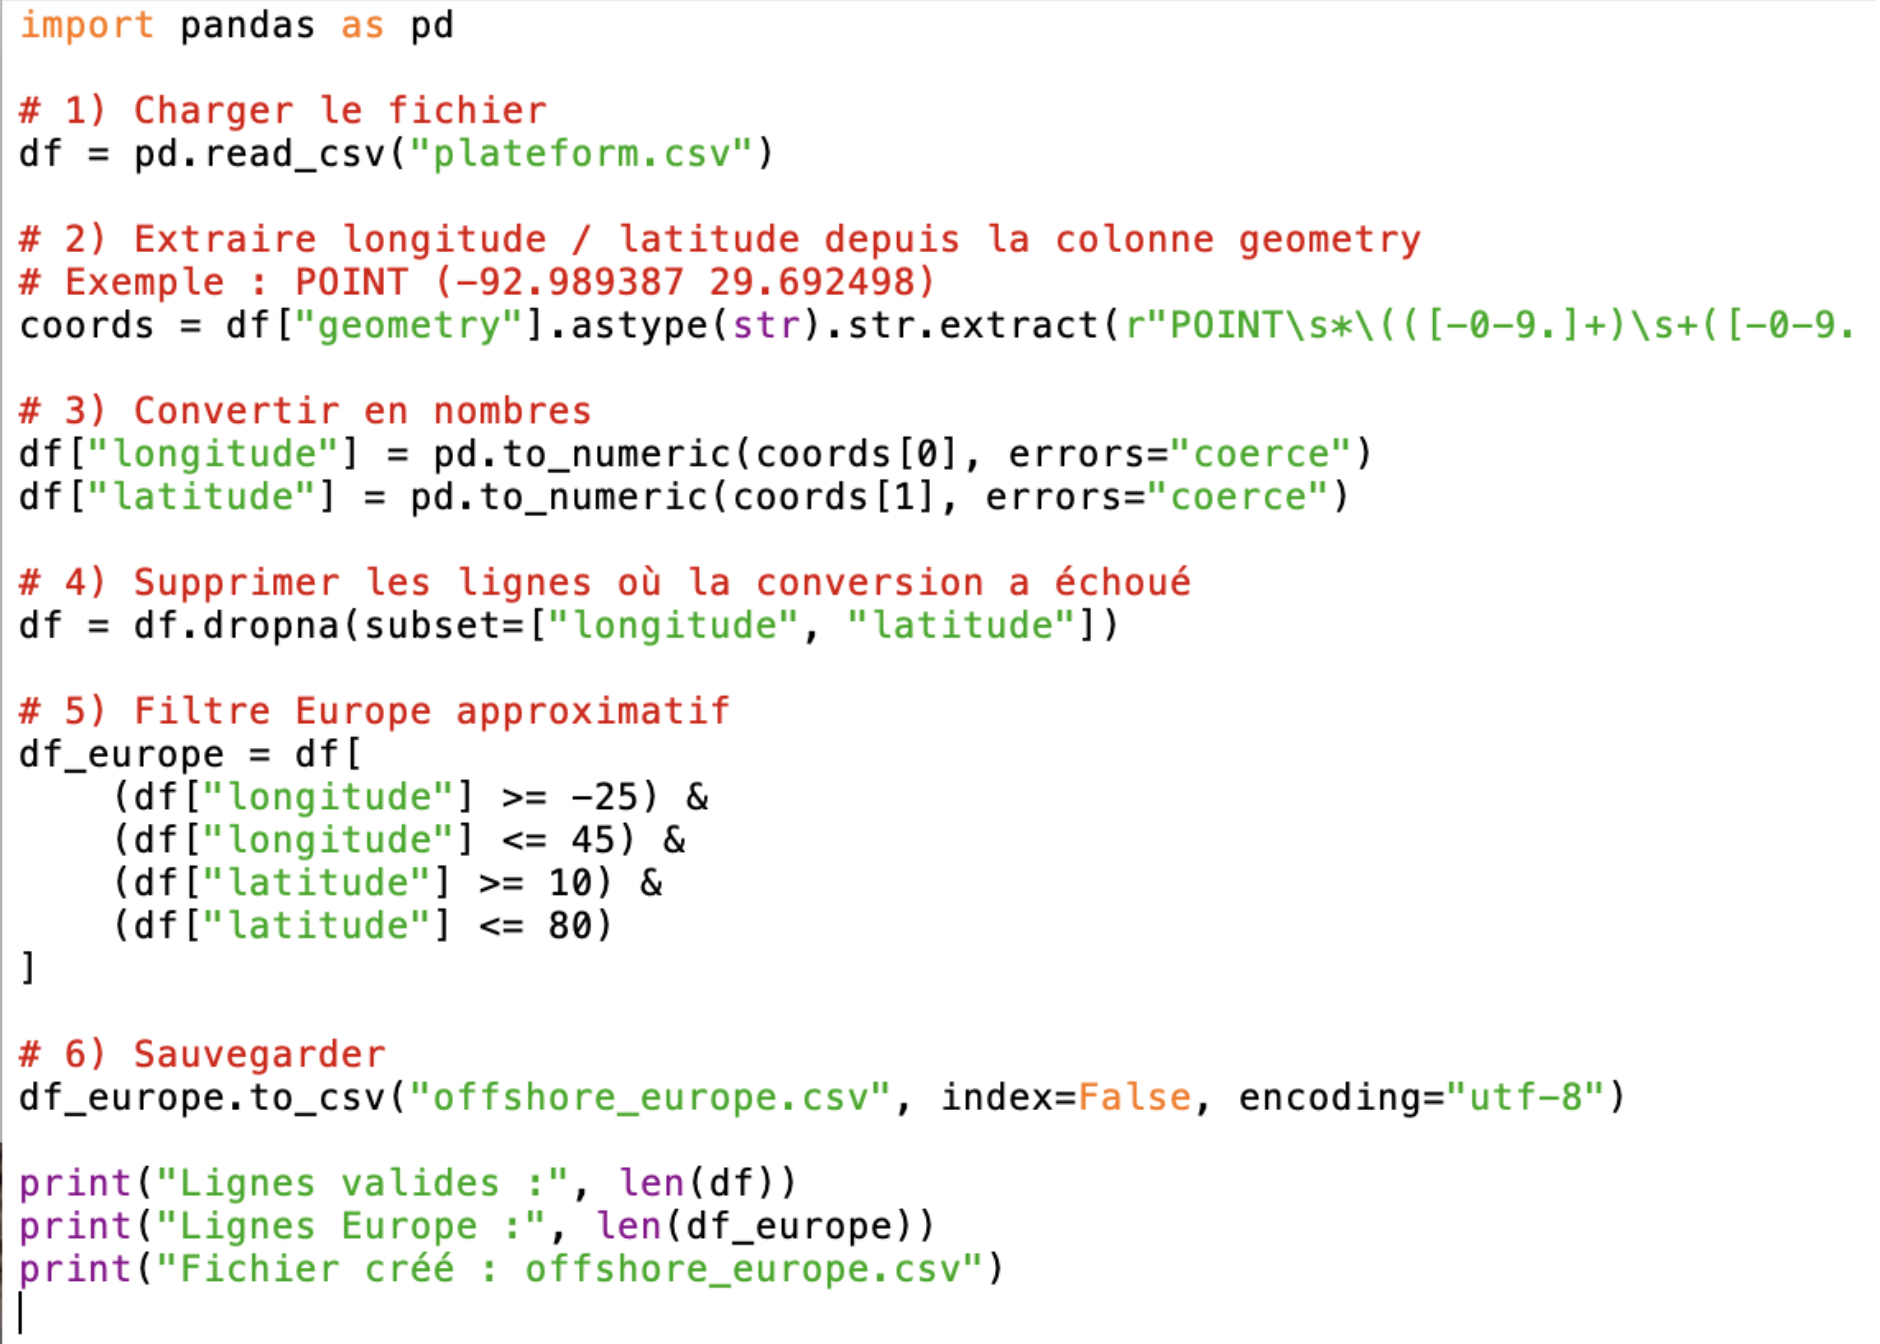
\includegraphics[width=7cm,height=\textheight,keepaspectratio]{scdon2-UPV-report-template_files/code.png}
\caption{Code.}\label{uml}
\end{figure}

Le fichier final obtenu est : \textbf{offshore\_europe.csv}

\subsection{Nettoyage des ports et
offshore}\label{nettoyage-des-ports-et-offshore}

Suppression des entrées sans coordonnées :

\begin{Shaded}
\begin{Highlighting}[]
\KeywordTok{DELETE} \KeywordTok{FROM}\NormalTok{ port\_maritime\_eur}
\KeywordTok{WHERE}\NormalTok{ latitude }\KeywordTok{IS} \KeywordTok{NULL} \KeywordTok{OR}\NormalTok{ longitude }\KeywordTok{IS} \KeywordTok{NULL}\NormalTok{;}
\end{Highlighting}
\end{Shaded}

\section{Calcul des distances}\label{calcul-des-distances}

\subsection{Ajout des variables de
distance}\label{ajout-des-variables-de-distance}

De nouvelles colonnes ont été ajoutées pour mesurer la proximité des
observations :

\begin{Shaded}
\begin{Highlighting}[]
\KeywordTok{ALTER} \KeywordTok{TABLE}\NormalTok{ observation\_europe}
\KeywordTok{ADD} \KeywordTok{COLUMN}\NormalTok{ distance\_port\_min }\DataTypeTok{DECIMAL}\NormalTok{(}\DecValTok{12}\NormalTok{,}\DecValTok{6}\NormalTok{),}
\KeywordTok{ADD} \KeywordTok{COLUMN}\NormalTok{ distance\_infra\_min }\DataTypeTok{DECIMAL}\NormalTok{(}\DecValTok{12}\NormalTok{,}\DecValTok{6}\NormalTok{),}
\KeywordTok{ADD} \KeywordTok{COLUMN}\NormalTok{ classe\_distance\_port }\DataTypeTok{VARCHAR}\NormalTok{(}\DecValTok{30}\NormalTok{),}
\KeywordTok{ADD} \KeywordTok{COLUMN}\NormalTok{ classe\_distance\_infra }\DataTypeTok{VARCHAR}\NormalTok{(}\DecValTok{30}\NormalTok{);}
\end{Highlighting}
\end{Shaded}

\subsection{Distance aux port et infrastructures
offshore}\label{distance-aux-port-et-infrastructures-offshore}

Nous avons utilisé une distance euclidienne simplifiée entre les
coordonnées de l'observation et celles des ports et fait de même pour
les infrastructures offshore:

\begin{Shaded}
\begin{Highlighting}[]
\KeywordTok{UPDATE}\NormalTok{ observation\_europe }
\KeywordTok{SET}\NormalTok{ distance\_infra\_min }\OperatorTok{=}\NormalTok{ (}
    \KeywordTok{SELECT} \FunctionTok{MIN}\NormalTok{(}
        \FunctionTok{SQRT}\NormalTok{(}
\NormalTok{            POW(observation\_europe.decimalLatitude }\OperatorTok{{-}}\NormalTok{ offshore\_europe.latitude, }\DecValTok{2}\NormalTok{) }\OperatorTok{+}
\NormalTok{            POW(observation\_europe.decimalLongitude }\OperatorTok{{-}}\NormalTok{ offshore\_europe.longitude, }\DecValTok{2}\NormalTok{)}
\NormalTok{        )}
\NormalTok{    )}
    \KeywordTok{FROM}\NormalTok{ offshore\_europe }
\NormalTok{);}
\end{Highlighting}
\end{Shaded}

\subsection{Construction des classes de
distance}\label{construction-des-classes-de-distance}

Les distances ont été regroupées en classes :

\begin{Shaded}
\begin{Highlighting}[]
\KeywordTok{UPDATE}\NormalTok{ observation\_europe}
\KeywordTok{SET}\NormalTok{ classe\_distance\_port }\OperatorTok{=}
    \ControlFlowTok{CASE}
        \ControlFlowTok{WHEN}\NormalTok{ distance\_port\_min }\OperatorTok{\textless{}} \FloatTok{0.01} \ControlFlowTok{THEN} \DecValTok{10}
        \ControlFlowTok{WHEN}\NormalTok{ distance\_port\_min }\OperatorTok{\textless{}} \FloatTok{0.02} \ControlFlowTok{THEN} \DecValTok{9}
        \ControlFlowTok{WHEN}\NormalTok{ distance\_port\_min }\OperatorTok{\textless{}} \FloatTok{0.03} \ControlFlowTok{THEN} \DecValTok{8}
        \ControlFlowTok{WHEN}\NormalTok{ distance\_port\_min }\OperatorTok{\textless{}} \FloatTok{0.05} \ControlFlowTok{THEN} \DecValTok{7}
        \ControlFlowTok{WHEN}\NormalTok{ distance\_port\_min }\OperatorTok{\textless{}} \FloatTok{0.07} \ControlFlowTok{THEN} \DecValTok{6}
        \ControlFlowTok{WHEN}\NormalTok{ distance\_port\_min }\OperatorTok{\textless{}} \FloatTok{0.10} \ControlFlowTok{THEN} \DecValTok{5}
        \ControlFlowTok{WHEN}\NormalTok{ distance\_port\_min }\OperatorTok{\textless{}} \FloatTok{0.15} \ControlFlowTok{THEN} \DecValTok{4}
        \ControlFlowTok{WHEN}\NormalTok{ distance\_port\_min }\OperatorTok{\textless{}} \FloatTok{0.20} \ControlFlowTok{THEN} \DecValTok{3}
        \ControlFlowTok{WHEN}\NormalTok{ distance\_port\_min }\OperatorTok{\textless{}} \FloatTok{0.30} \ControlFlowTok{THEN} \DecValTok{2}
        \ControlFlowTok{ELSE} \DecValTok{1}
    \ControlFlowTok{END}\NormalTok{;}
\end{Highlighting}
\end{Shaded}

\subsection{Liaison avec les infrastructures
offshore}\label{liaison-avec-les-infrastructures-offshore}

On crée alors une liaison entre les 2 en ajoutant le port le plus proche
et en liant les collones en FK.

\begin{Shaded}
\begin{Highlighting}[]
\KeywordTok{UPDATE}\NormalTok{ observation\_europe o}
\KeywordTok{SET}\NormalTok{ id\_offshore\_proche }\OperatorTok{=}\NormalTok{ (}
    \KeywordTok{SELECT}\NormalTok{ i.id\_offshore}
    \KeywordTok{FROM}\NormalTok{ offshore\_europe i}
    \KeywordTok{ORDER} \KeywordTok{BY} 
\NormalTok{        ((o.decimalLatitude }\OperatorTok{{-}}\NormalTok{ i.latitude) }\OperatorTok{*}\NormalTok{ (o.decimalLatitude }\OperatorTok{{-}}\NormalTok{ i.latitude)) }\OperatorTok{+}
\NormalTok{        ((o.decimalLongitude }\OperatorTok{{-}}\NormalTok{ i.longitude) }\OperatorTok{*}\NormalTok{ (o.decimalLongitude }\OperatorTok{{-}}\NormalTok{ i.longitude))}
    \KeywordTok{LIMIT} \DecValTok{1}
\NormalTok{);}
\end{Highlighting}
\end{Shaded}

Ajout de la clé étrangère :

\begin{Shaded}
\begin{Highlighting}[]
\KeywordTok{ALTER} \KeywordTok{TABLE}\NormalTok{ observation\_europe}
\KeywordTok{ADD} \KeywordTok{CONSTRAINT}\NormalTok{ fk\_obs\_offshore}
\KeywordTok{FOREIGN} \KeywordTok{KEY}\NormalTok{ (id\_offshore\_proche) }\KeywordTok{REFERENCES}\NormalTok{ offshore\_europe(id\_offshore);}
\end{Highlighting}
\end{Shaded}

\begin{center}\rule{0.5\linewidth}{0.5pt}\end{center}

\section{Analyse des données}\label{analyse-des-donnuxe9es}

L'objectif de cette analyse est d'étudier l'influence de la proximité
aux ports sur la répartition des observations biologiques.

\subsection{Distance moyenne au port par
phylum}\label{distance-moyenne-au-port-par-phylum}

Cette requête permet de calculer la distance moyenne des observations
par phylum, afin d'identifier les groupes biologiques les plus proches
ou éloignés des infrastructures portuaires.

\begin{Shaded}
\begin{Highlighting}[]
\KeywordTok{SELECT}\NormalTok{ phylum, }\FunctionTok{AVG}\NormalTok{(distance\_port\_min) }\KeywordTok{AS}\NormalTok{ distance\_port\_moyenne}
\KeywordTok{FROM}\NormalTok{ observation\_europe}
\KeywordTok{GROUP} \KeywordTok{BY}\NormalTok{ phylum;}
\end{Highlighting}
\end{Shaded}

\begin{figure}
\centering
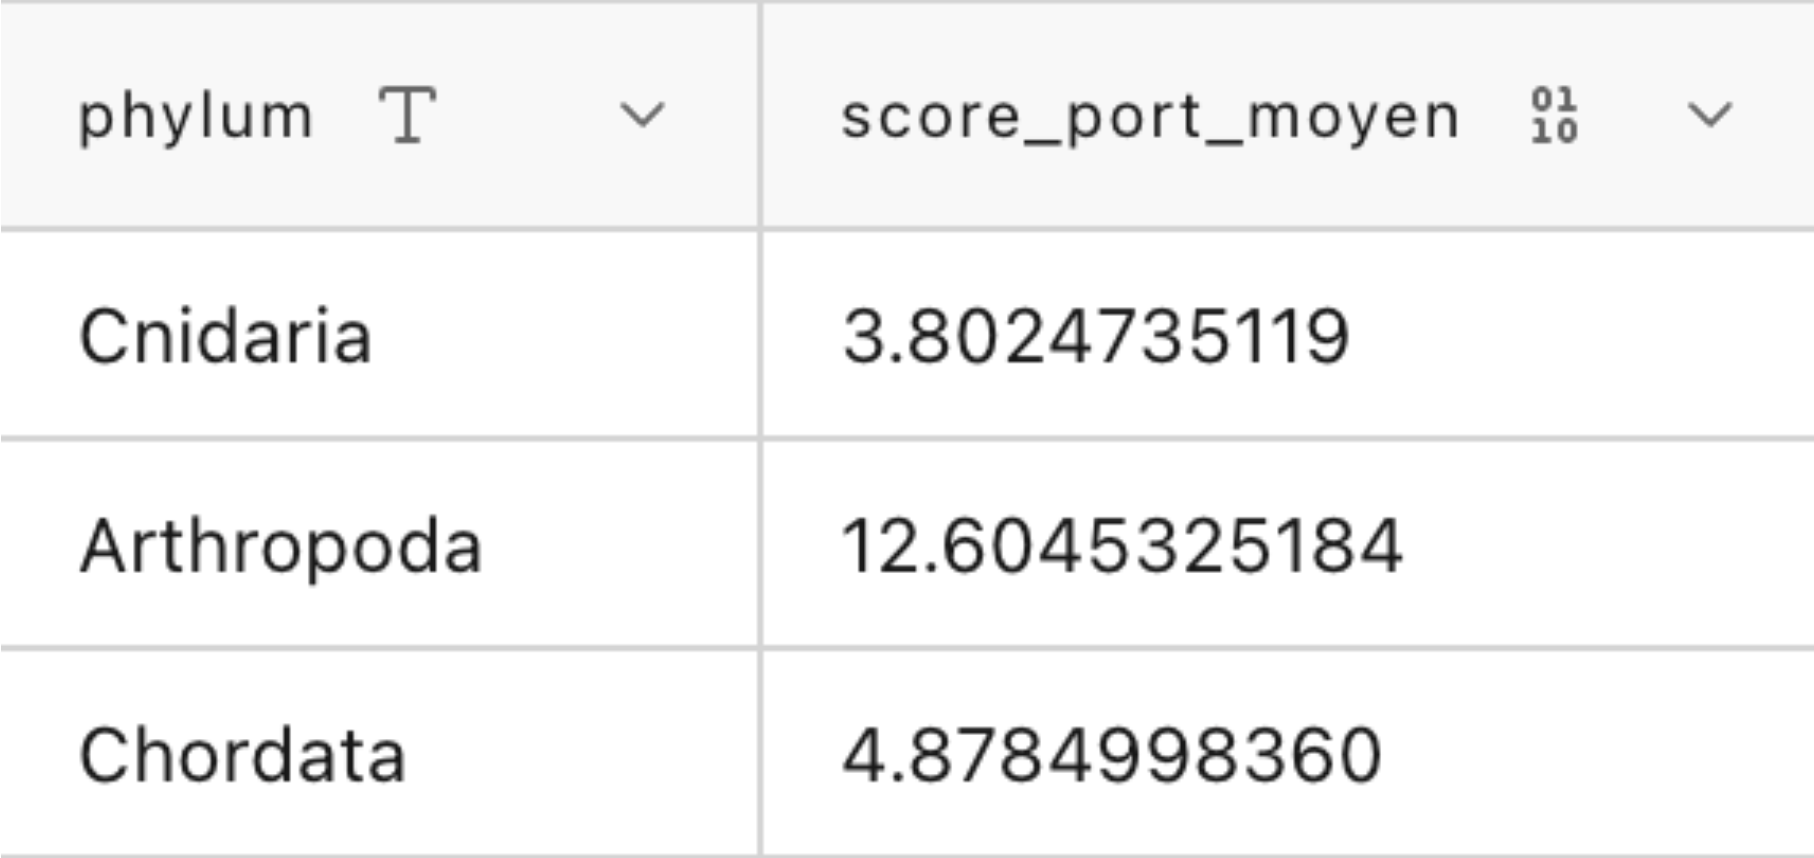
\includegraphics[width=7cm,height=\textheight,keepaspectratio]{scdon2-UPV-report-template_files/dist.png}
\caption{Code.}\label{uml}
\end{figure}

\subsection{Répartition des observations selon la distance au
port}\label{ruxe9partition-des-observations-selon-la-distance-au-port}

On analyse ici le nombre d'observations en fonction des classes de
distance aux ports, ce qui permet de visualiser la distribution spatiale
des données.

\begin{Shaded}
\begin{Highlighting}[]
\KeywordTok{SELECT}\NormalTok{ classe\_distance\_port, }\FunctionTok{COUNT}\NormalTok{(}\OperatorTok{*}\NormalTok{) }\KeywordTok{AS}\NormalTok{ nb\_observations}
\KeywordTok{FROM}\NormalTok{ observation\_europe}
\KeywordTok{GROUP} \KeywordTok{BY}\NormalTok{ classe\_distance\_port}
\KeywordTok{ORDER} \KeywordTok{BY}\NormalTok{ classe\_distance\_port;}
\end{Highlighting}
\end{Shaded}

\begin{figure}
\centering
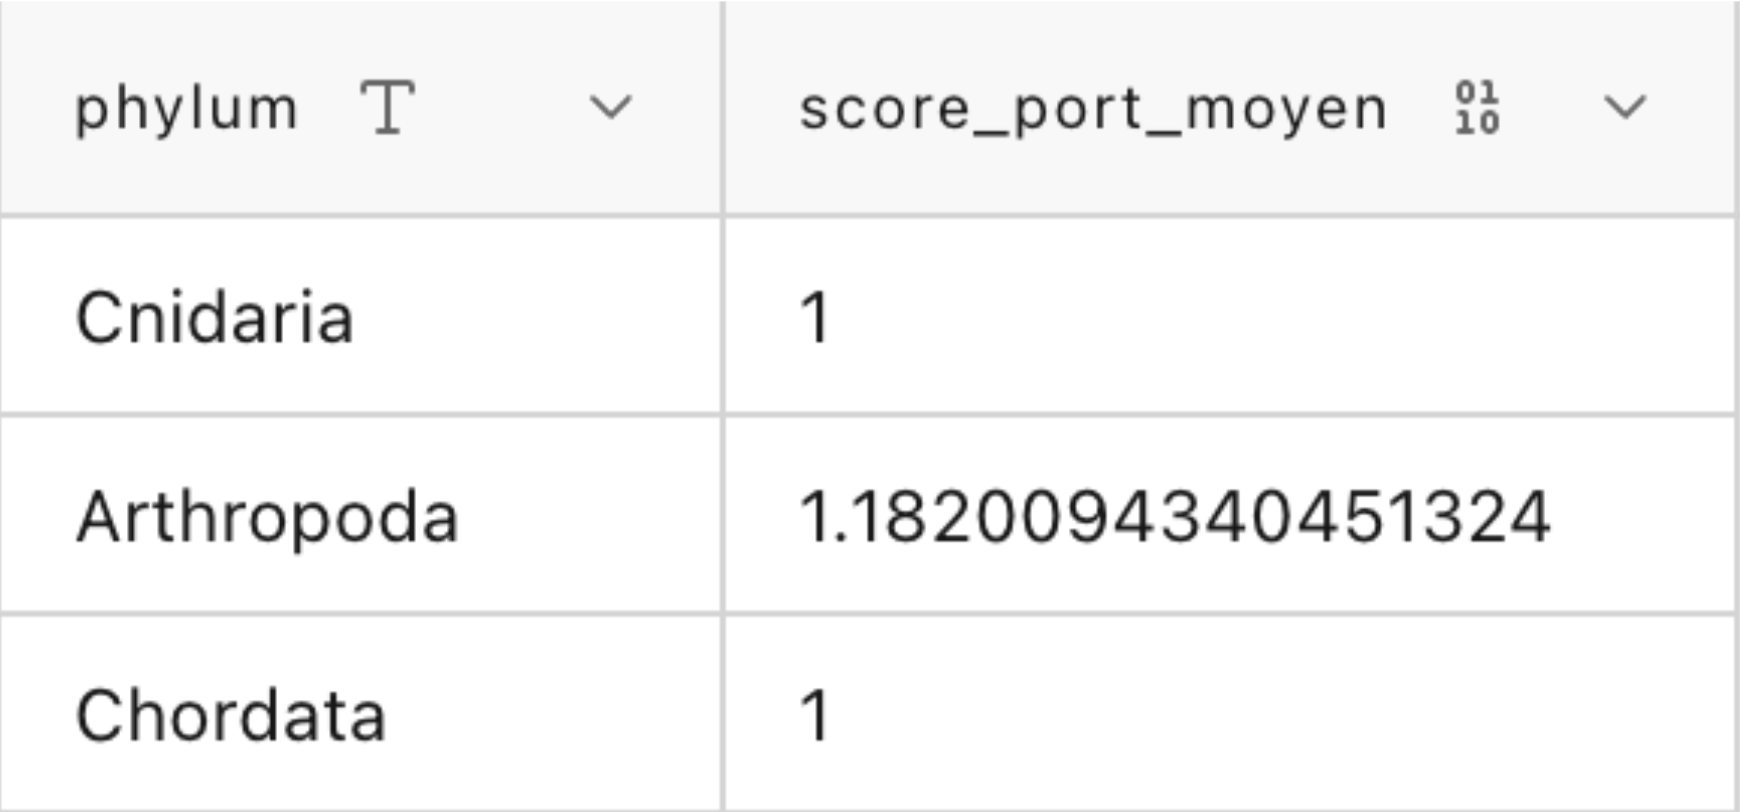
\includegraphics[width=7cm,height=\textheight,keepaspectratio]{scdon2-UPV-report-template_files/diff.png}
\caption{Code.}\label{uml}
\end{figure}

\subsection{Nombre d'espèces distinctes selon la distance au
port}\label{nombre-despuxe8ces-distinctes-selon-la-distance-au-port}

Cette requête met en évidence la pression exercée par les
infrastructures

\begin{Shaded}
\begin{Highlighting}[]
\KeywordTok{SELECT}\NormalTok{ classe\_distance\_port, }\FunctionTok{COUNT}\NormalTok{(}\KeywordTok{DISTINCT}\NormalTok{ species) }\KeywordTok{AS}\NormalTok{ nb\_especes\_distinctes}
\KeywordTok{FROM}\NormalTok{ observation\_europe}
\KeywordTok{WHERE}\NormalTok{ species }\KeywordTok{IS} \KeywordTok{NOT} \KeywordTok{NULL}
\KeywordTok{GROUP} \KeywordTok{BY}\NormalTok{ classe\_distance\_port}
\KeywordTok{ORDER} \KeywordTok{BY}\NormalTok{ classe\_distance\_port;}
\end{Highlighting}
\end{Shaded}

\begin{figure}
\centering
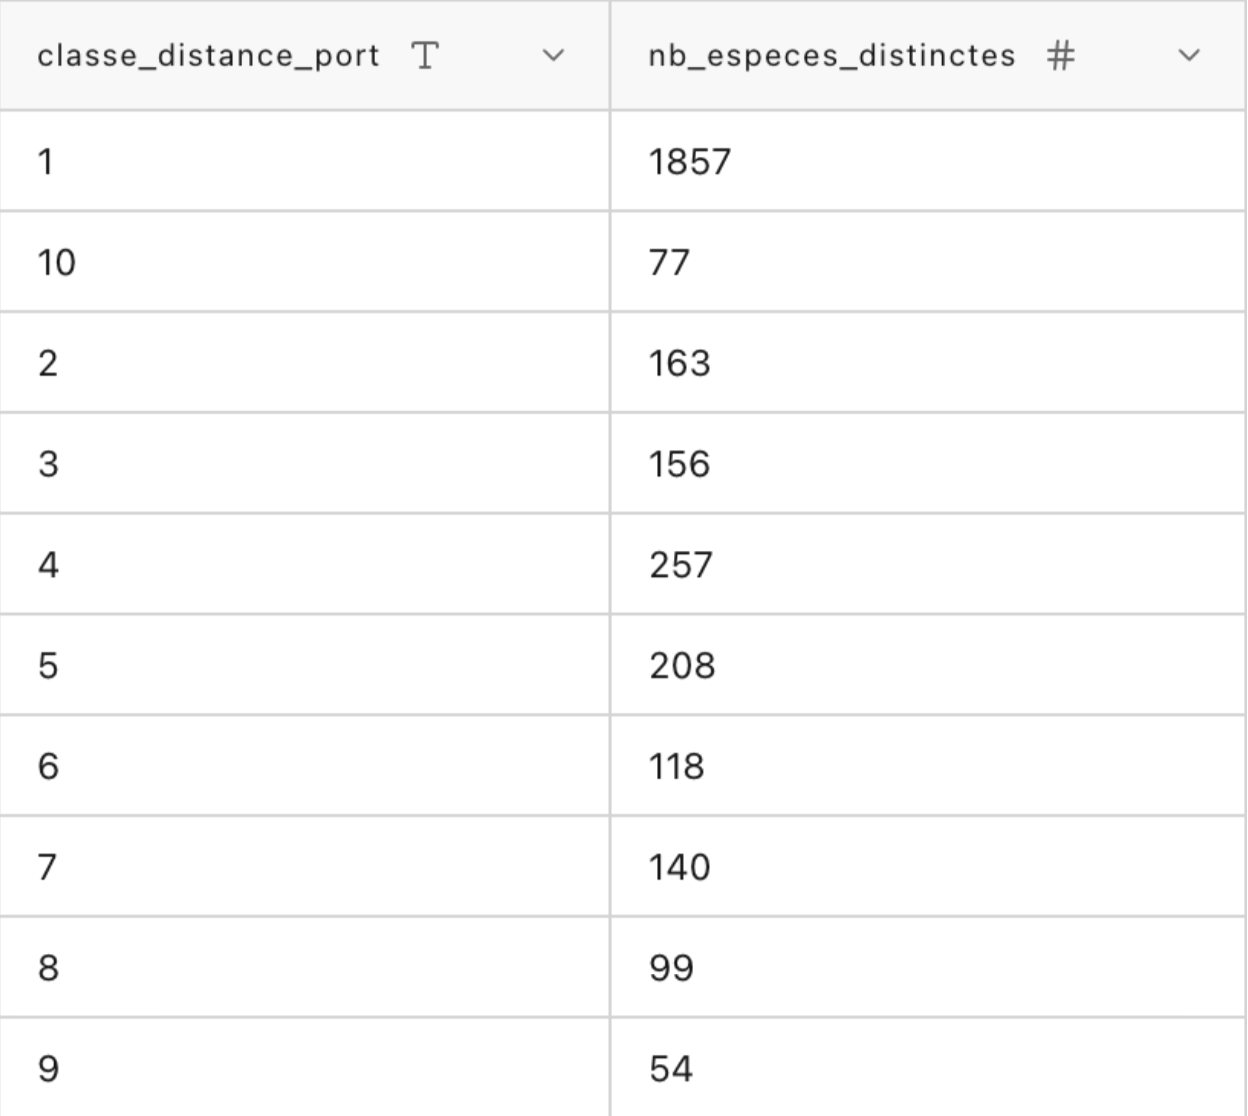
\includegraphics[width=7cm,height=\textheight,keepaspectratio]{scdon2-UPV-report-template_files/impact.png}
\caption{Code.}\label{uml}
\end{figure}

\subsection{Distance moyenne au port par classe
taxonomique}\label{distance-moyenne-au-port-par-classe-taxonomique}

Analyse de la distance moyenne aux ports selon les classes taxonomiques.

\begin{Shaded}
\begin{Highlighting}[]
\KeywordTok{SELECT}\NormalTok{ \textasciigrave{}class\textasciigrave{}, }\FunctionTok{AVG}\NormalTok{(distance\_port\_min) }\KeywordTok{AS}\NormalTok{ distance\_port\_moyenne}
\KeywordTok{FROM}\NormalTok{ observation\_europe}
\KeywordTok{WHERE}\NormalTok{ \textasciigrave{}class\textasciigrave{} }\KeywordTok{IS} \KeywordTok{NOT} \KeywordTok{NULL}
\KeywordTok{GROUP} \KeywordTok{BY}\NormalTok{ \textasciigrave{}class\textasciigrave{}}
\KeywordTok{ORDER} \KeywordTok{BY}\NormalTok{ distance\_port\_moyenne;}
\end{Highlighting}
\end{Shaded}

\begin{figure}
\centering
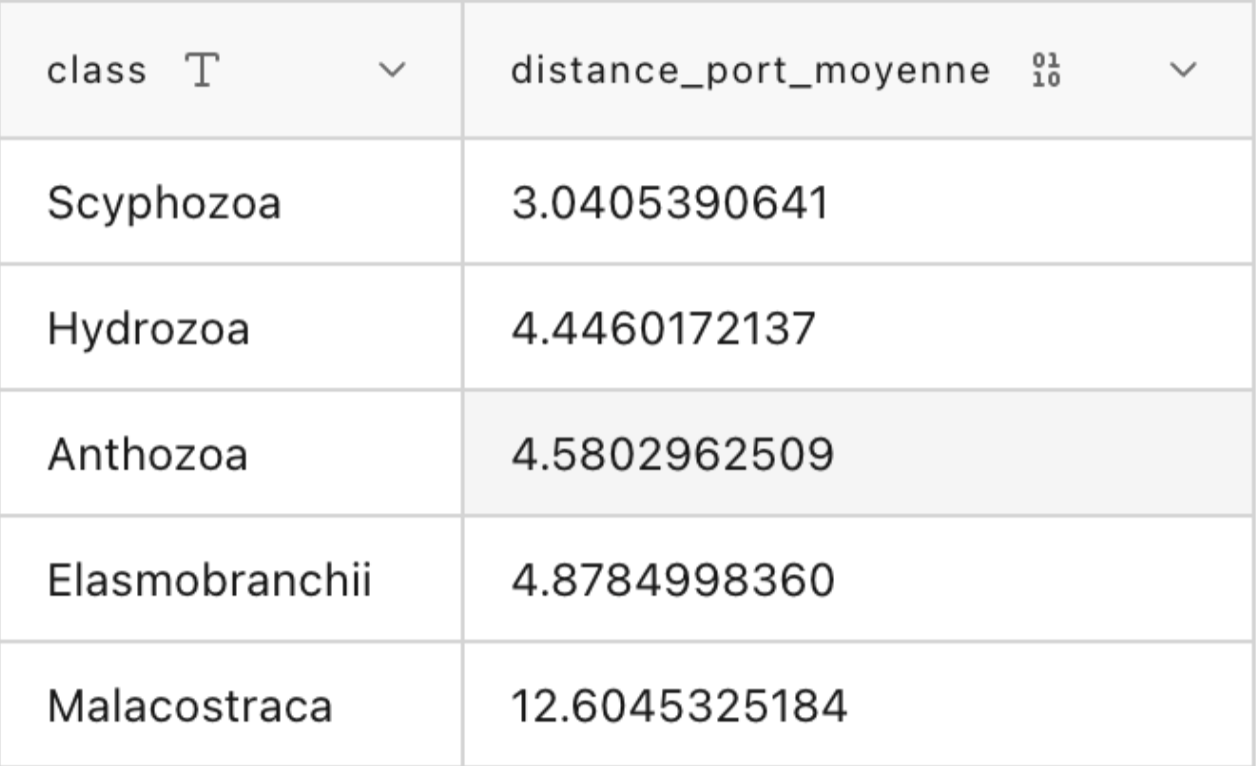
\includegraphics[width=7cm,height=\textheight,keepaspectratio]{scdon2-UPV-report-template_files/taxo.png}
\caption{Code.}\label{uml}
\end{figure}

\subsection{Espèces les plus observées à proximité immédiate des
ports}\label{espuxe8ces-les-plus-observuxe9es-uxe0-proximituxe9-immuxe9diate-des-ports}

Identification des espèces les plus fréquentes dans les zones très
proches des ports (classe 10).

\begin{Shaded}
\begin{Highlighting}[]
\KeywordTok{SELECT}\NormalTok{ species, }\FunctionTok{COUNT}\NormalTok{(}\OperatorTok{*}\NormalTok{) }\KeywordTok{AS}\NormalTok{ nb\_observations}
\KeywordTok{FROM}\NormalTok{ observation\_europe}
\KeywordTok{WHERE}\NormalTok{ species }\KeywordTok{IS} \KeywordTok{NOT} \KeywordTok{NULL}
  \KeywordTok{AND}\NormalTok{ classe\_distance\_port }\OperatorTok{=} \DecValTok{10}
\KeywordTok{GROUP} \KeywordTok{BY}\NormalTok{ species}
\KeywordTok{ORDER} \KeywordTok{BY}\NormalTok{ nb\_observations }\KeywordTok{DESC}
\KeywordTok{LIMIT} \DecValTok{20}\NormalTok{;}
\end{Highlighting}
\end{Shaded}

\subsection{Espèces les plus observées loin des
ports}\label{espuxe8ces-les-plus-observuxe9es-loin-des-ports}

Analyse équivalente pour les zones les plus éloignées des ports (classe
1).

\begin{Shaded}
\begin{Highlighting}[]
\KeywordTok{SELECT}\NormalTok{ species, }\FunctionTok{COUNT}\NormalTok{(}\OperatorTok{*}\NormalTok{) }\KeywordTok{AS}\NormalTok{ nb\_observations}
\KeywordTok{FROM}\NormalTok{ observation\_europe}
\KeywordTok{WHERE}\NormalTok{ species }\KeywordTok{IS} \KeywordTok{NOT} \KeywordTok{NULL}
  \KeywordTok{AND}\NormalTok{ classe\_distance\_port }\OperatorTok{=} \DecValTok{1}
\KeywordTok{GROUP} \KeywordTok{BY}\NormalTok{ species}
\KeywordTok{ORDER} \KeywordTok{BY}\NormalTok{ nb\_observations }\KeywordTok{DESC}
\KeywordTok{LIMIT} \DecValTok{20}\NormalTok{;}
\end{Highlighting}
\end{Shaded}

\subsection{Nombre d'observations par
année}\label{nombre-dobservations-par-annuxe9e}

Permet d'étudier l'évolution temporelle du nombre d'observations.

\begin{Shaded}
\begin{Highlighting}[]
\KeywordTok{SELECT}\NormalTok{ \textasciigrave{}year\textasciigrave{}, }\FunctionTok{COUNT}\NormalTok{(}\OperatorTok{*}\NormalTok{) }\KeywordTok{AS}\NormalTok{ nb\_observations}
\KeywordTok{FROM}\NormalTok{ observation\_europe}
\KeywordTok{GROUP} \KeywordTok{BY}\NormalTok{ \textasciigrave{}year\textasciigrave{}}
\KeywordTok{ORDER} \KeywordTok{BY}\NormalTok{ \textasciigrave{}year\textasciigrave{};}
\end{Highlighting}
\end{Shaded}

\begin{figure}
\centering
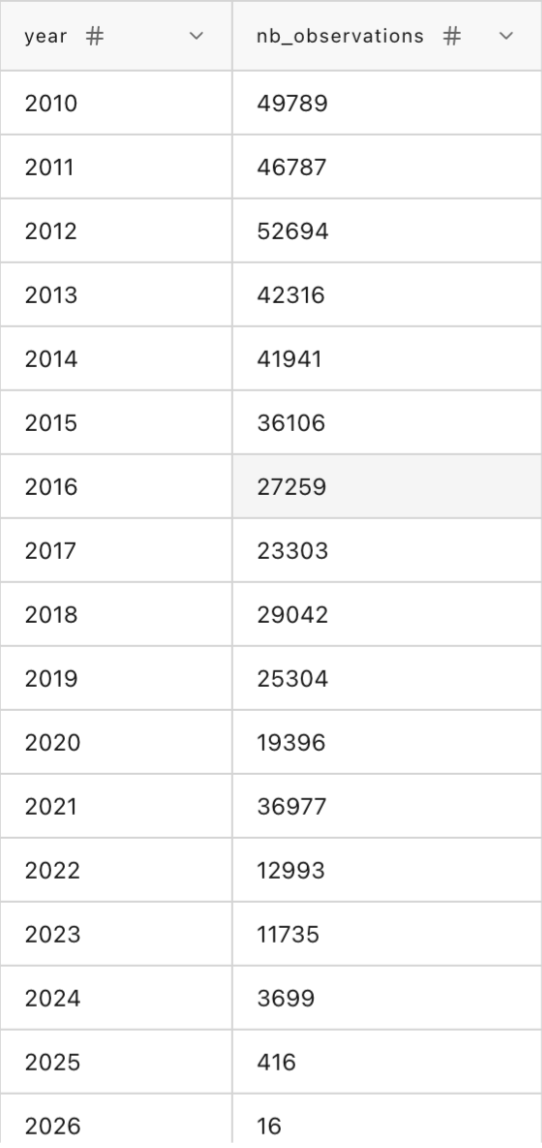
\includegraphics[width=7cm,height=\textheight,keepaspectratio]{scdon2-UPV-report-template_files/annee.png}
\caption{Code.}\label{uml}
\end{figure}

\subsection{Phylums proches des ports avec un nombre significatif
d'observations}\label{phylums-proches-des-ports-avec-un-nombre-significatif-dobservations}

On sélectionne les phylums ayant au moins 20 observations afin d'assurer
une certaine robustesse statistique.

\begin{Shaded}
\begin{Highlighting}[]
\KeywordTok{SELECT}\NormalTok{ phylum,}
       \FunctionTok{AVG}\NormalTok{(distance\_port\_min) }\KeywordTok{AS}\NormalTok{ distance\_port\_moyenne,}
       \FunctionTok{COUNT}\NormalTok{(}\OperatorTok{*}\NormalTok{) }\KeywordTok{AS}\NormalTok{ nb\_observations}
\KeywordTok{FROM}\NormalTok{ observation\_europe}
\KeywordTok{WHERE}\NormalTok{ phylum }\KeywordTok{IS} \KeywordTok{NOT} \KeywordTok{NULL}
\KeywordTok{GROUP} \KeywordTok{BY}\NormalTok{ phylum}
\KeywordTok{HAVING} \FunctionTok{COUNT}\NormalTok{(}\OperatorTok{*}\NormalTok{) }\OperatorTok{\textgreater{}=} \DecValTok{20}
\KeywordTok{ORDER} \KeywordTok{BY}\NormalTok{ distance\_port\_moyenne }\KeywordTok{ASC}\NormalTok{;}
\end{Highlighting}
\end{Shaded}

\begin{figure}
\centering
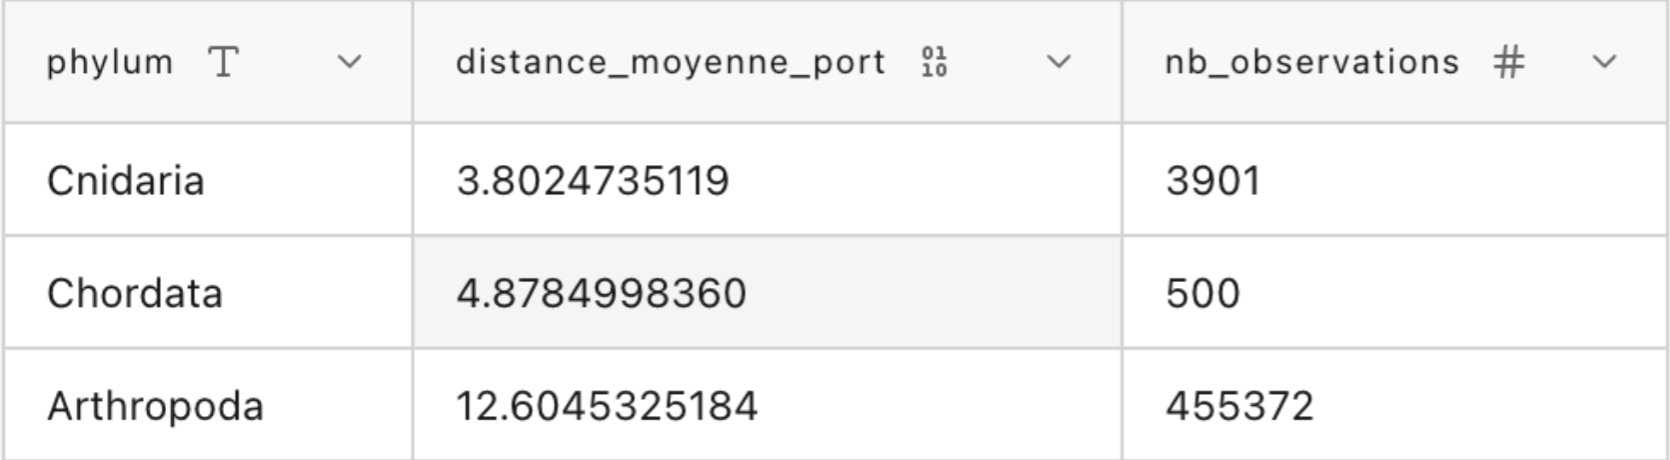
\includegraphics[width=7cm,height=\textheight,keepaspectratio]{scdon2-UPV-report-template_files/phy.png}
\caption{Code.}\label{uml}
\end{figure}

\subsection{Association des observations avec le port le plus
proche}\label{association-des-observations-avec-le-port-le-plus-proche}

Jointure entre les observations et la table des ports pour récupérer le
nom du port le plus proche.

\begin{Shaded}
\begin{Highlighting}[]
\KeywordTok{SELECT} 
\NormalTok{    o.id\_observation,}
\NormalTok{    o.species,}
\NormalTok{    o.distance\_port\_min,}
\NormalTok{    p.nomport}
\KeywordTok{FROM}\NormalTok{ observation\_europe o}
\KeywordTok{INNER} \KeywordTok{JOIN}\NormalTok{ port\_maritime\_eur p}
    \KeywordTok{ON}\NormalTok{ o.gid\_port\_proche }\OperatorTok{=}\NormalTok{ p.gid;}
\end{Highlighting}
\end{Shaded}

\subsection{Observations situées à une distance inférieure à la
moyenne}\label{observations-situuxe9es-uxe0-une-distance-infuxe9rieure-uxe0-la-moyenne}

Sélection des observations plus proches des ports que la moyenne
globale.

\begin{Shaded}
\begin{Highlighting}[]
\KeywordTok{SELECT} 
\NormalTok{    id\_observation,}
\NormalTok{    species,}
\NormalTok{    distance\_port\_min}
\KeywordTok{FROM}\NormalTok{ observation\_europe}
\KeywordTok{WHERE}\NormalTok{ distance\_port\_min }\OperatorTok{\textless{}}\NormalTok{ (}
    \KeywordTok{SELECT} \FunctionTok{AVG}\NormalTok{(distance\_port\_min)}
    \KeywordTok{FROM}\NormalTok{ observation\_europe}
\NormalTok{);}
\end{Highlighting}
\end{Shaded}

\subsection{Phylums abondants et proches des
ports}\label{phylums-abondants-et-proches-des-ports}

Identification des phylums ayant un nombre important d'observations
(\textgreater= 100) et une distance moyenne faible aux ports.

\begin{Shaded}
\begin{Highlighting}[]
\KeywordTok{SELECT} 
\NormalTok{    phylum,}
    \FunctionTok{COUNT}\NormalTok{(}\OperatorTok{*}\NormalTok{) }\KeywordTok{AS}\NormalTok{ nb\_observations,}
    \FunctionTok{AVG}\NormalTok{(distance\_port\_min) }\KeywordTok{AS}\NormalTok{ distance\_port\_moyenne}
\KeywordTok{FROM}\NormalTok{ observation\_europe}
\KeywordTok{WHERE}\NormalTok{ phylum }\KeywordTok{IS} \KeywordTok{NOT} \KeywordTok{NULL}
\KeywordTok{GROUP} \KeywordTok{BY}\NormalTok{ phylum}
\KeywordTok{HAVING} \FunctionTok{COUNT}\NormalTok{(}\OperatorTok{*}\NormalTok{) }\OperatorTok{\textgreater{}=} \DecValTok{100}
\KeywordTok{ORDER} \KeywordTok{BY}\NormalTok{ distance\_port\_moyenne }\KeywordTok{ASC}\NormalTok{;}
\end{Highlighting}
\end{Shaded}

\begin{figure}
\centering
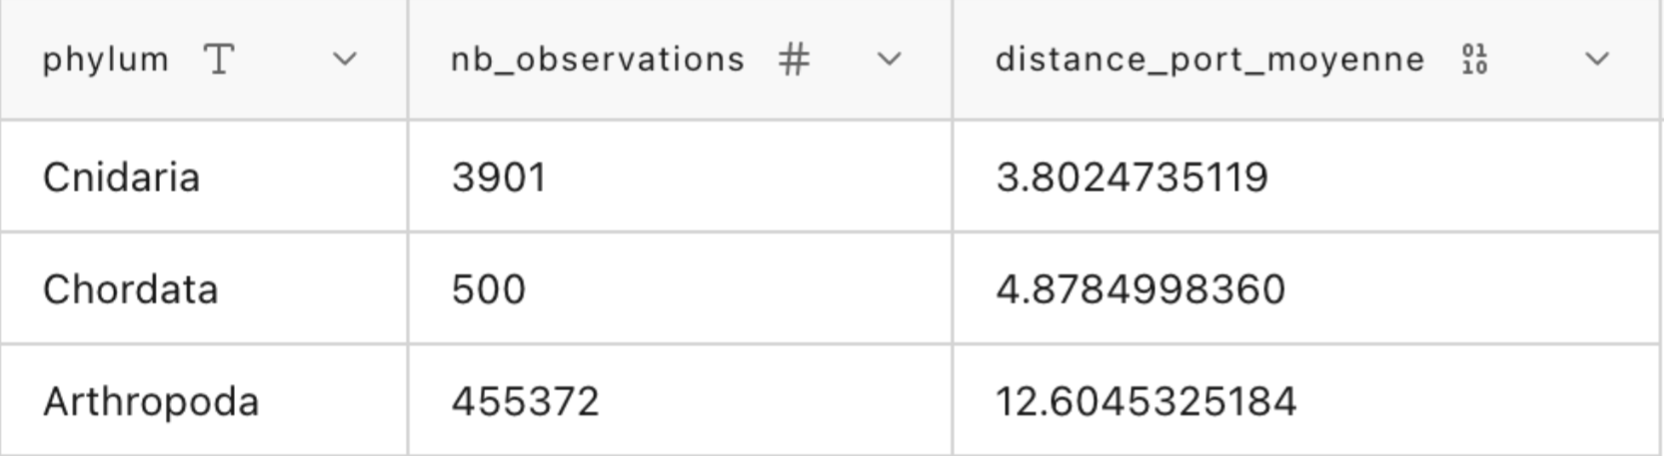
\includegraphics[width=7cm,height=\textheight,keepaspectratio]{scdon2-UPV-report-template_files/abond.png}
\caption{Code.}\label{uml}
\end{figure}

\section{Quelques détails
techniques}\label{quelques-duxe9tails-techniques}

On peut interagir avec une base de données directement depuis RMarkdown
: i.e.~requêter puis récupérer et afficher le résultat directement
depuis le Rmd. Un fichier connexionBDD.Rmd est fourni pour donner des
exemples.

\chapter{Matériel et Méthodes}\label{matuxe9riel-et-muxe9thodes}

\section{Logiciels}\label{logiciels}

Lister tous les logiciels utilisés pour la partie statistique du rapport
(et également ceux pour gérer et communiquer entre les membres du projet
s'il y en a en particulier)

\medskip

R (ou Python) est le logiciel à privilégier pour la Science des Données.
Pour assurer une reproductibilité maximale, vous devriez utiliser R
Markdown (ou un Notebook Jupyter, et éventuellement un outil de gestion
des versions tel que \texttt{Git}), par exemple via Google Colab ou
RStudio dans les nuages. Évitez d'utiliser Word!

\bigskip

Il est de votre responsabilité de donner les versions des logiciels que
vous utilisez, ainsi que de donner des informations techniques sur
l'ordinateur qui vous a servi pour les analyses (système d'exploitation,
vitesse du processeur, etc.). Penser à fournir des citations pour les
logiciels utilisés, par exemple
\footnote{L'entrée BibTeX ajoutée dans le fichier \texttt{references.bib} a été obtenue grâce à la commande  \texttt{citation(package = "tidyverse")} tapée dans la console de R.}.

\section{Modélisation statistique}\label{moduxe9lisation-statistique}

Quels outils ou méthodes de statistiques allez-vous utiliser? Donner des
équations mathématiques s'il y a lieu et lister les éventuels
présupposés («assumptions» en anglais) que vous devez faire sur les
données afin d'utiliser ces outils ou méthodes (\emph{e.g.}, normalité,
absence de valeurs aberrantes, etc.).

Il est également bon d'indiquer quelles sont les avantages et les
limites de ces méthodes.

Vous pourrez consulter avec profit les Chapitre 11--13 du livre sur R :

\url{http://biostatisticien.eu/springeR/livreR.pdf}

\chapter{Analyse Exploratoire des
Données}\label{analyse-exploratoire-des-donnuxe9es}

Toute étude impliquant des données doit \textbf{obligatoirement} inclure
une analyse exploratoire préalable. Celle-ci permet de mieux comprendre
l'information contenue dans les données.

Il faut produire de nombreux résumés graphiques (\emph{e.g.},
histogrammes, nuages de points, boxplots, etc.) et numériques
(\emph{e.g.}, médiane, moyenne, variance, etc.). Ainsi, il faut faire
une analyse descriptive uni- et bivariée systématique de toutes les
variables du jeu de données. Puis, il faut uniquement conserver les plus
pertinents (les autres pouvant être gardés en Annexe), c'est-à-dire ceux
qui permettront de dégager des éléments de réponse pour la question de
recherche envisagée. Chaque figure et tableau doit être commenté. Mais
il ne faut pas extrapoler et dire des choses qui ne sont pas visibles
dans ces graphiques ou tableaux. Pour chaque analyse, vous pourrez
préciser le nombre d'individus/ d'unités statistiques concernés au
total.

Vous pourrez consulter avec profit le Chapitre 9 du livre sur R :

\url{http://biostatisticien.eu/springeR/livreR.pdf}

\section{Utiliser R}\label{utiliser-r}

Il est facile d'inclure des codes R dans votre rapport, qui seront
exécutés à la volée (\emph{i.e.}, lors de la traduction de votre fichier
\texttt{Rmd} en fichier \texttt{PDF} ou \texttt{DOC}). Par exemple:

\begin{Shaded}
\begin{Highlighting}[]
\FunctionTok{boxplot}\NormalTok{(cars, }\AttributeTok{col =} \FunctionTok{c}\NormalTok{(}\StringTok{"\#5975a4"}\NormalTok{, }\StringTok{"\#cc8963"}\NormalTok{))}
\end{Highlighting}
\end{Shaded}

\begin{figure}

{\centering 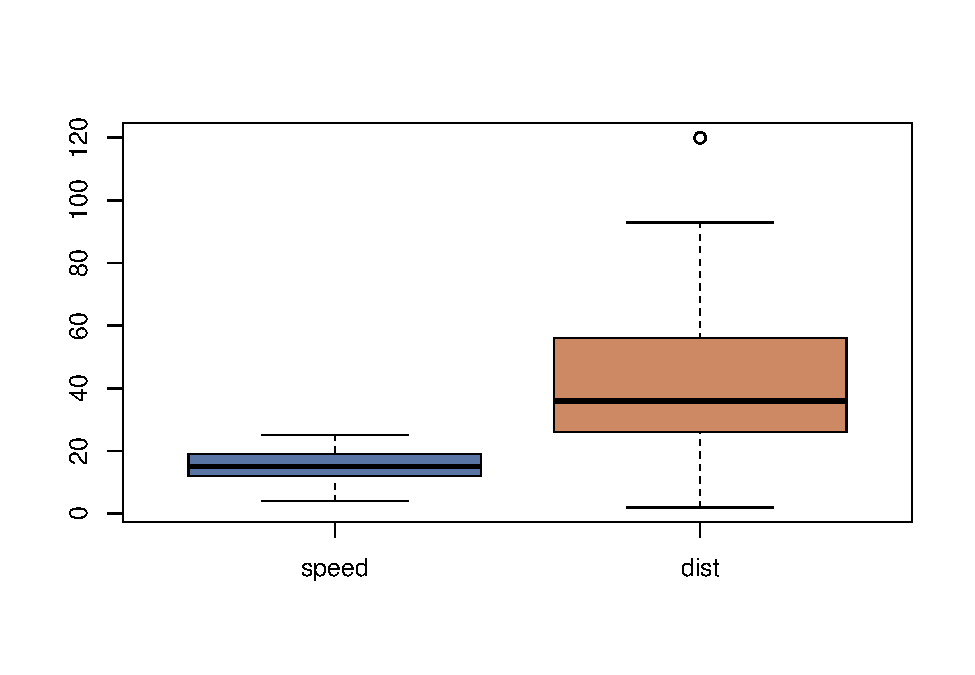
\includegraphics[width=7cm]{scdon2-UPV-report-template_files/figure-latex/unnamed-chunk-1-1} 

}

\caption{\label{fig:boxplots}Deux boxplots.}\label{fig:unnamed-chunk-1}
\end{figure}

\begin{Shaded}
\begin{Highlighting}[]
\FunctionTok{colMeans}\NormalTok{(cars)}
\end{Highlighting}
\end{Shaded}

\begin{verbatim}
## speed  dist 
## 15.40 42.98
\end{verbatim}

Les lignes de code ne doivent pas dépasser dans la marge de droite.
Ainsi on pourrait remplacer le chunk ci-dessous:

\begin{Shaded}
\begin{Highlighting}[]
\FunctionTok{boxplot}\NormalTok{(cars, }\AttributeTok{main =} \StringTok{"Un titre qui est vraiment beaucoup trop long et qui dépasse dans la marge de droite"}\NormalTok{)}
\end{Highlighting}
\end{Shaded}

\begin{figure}

{\centering 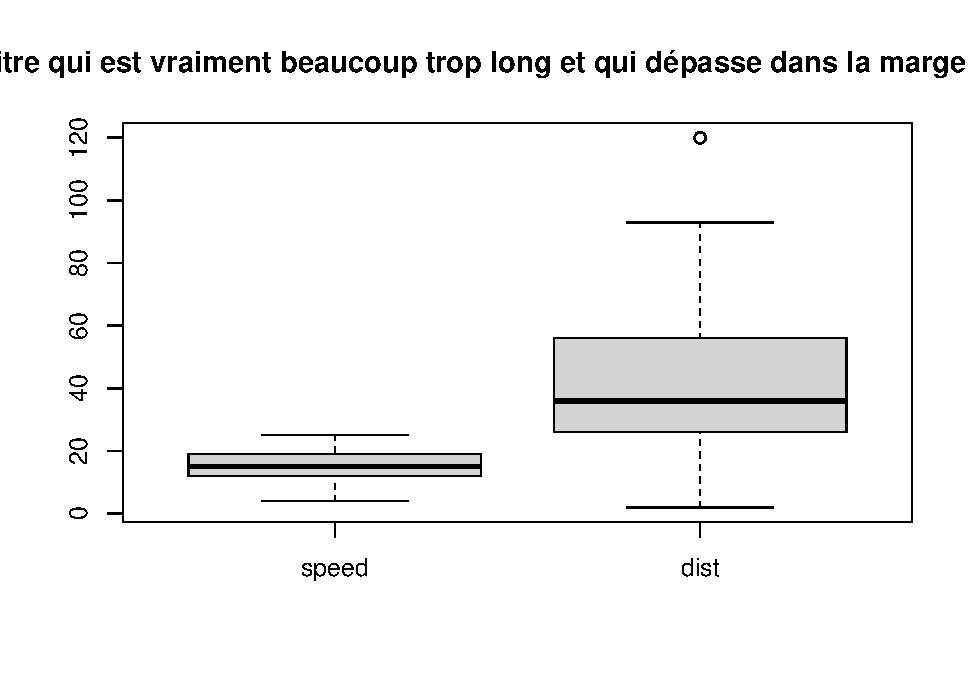
\includegraphics[width=7cm]{scdon2-UPV-report-template_files/figure-latex/unnamed-chunk-2-1} 

}

\caption{Pas super.}\label{fig:unnamed-chunk-2}
\end{figure}

par celui-ci:

\tiny

\begin{Shaded}
\begin{Highlighting}[]
\FunctionTok{boxplot}\NormalTok{(cars, }
        \AttributeTok{main =} \StringTok{"Un titre qui est vraiment beaucoup trop long}\SpecialCharTok{\textbackslash{}n}\StringTok{ mais qui ne dépasse plus dans la marge de droite"}\NormalTok{)}
\end{Highlighting}
\end{Shaded}

\begin{figure}

{\centering 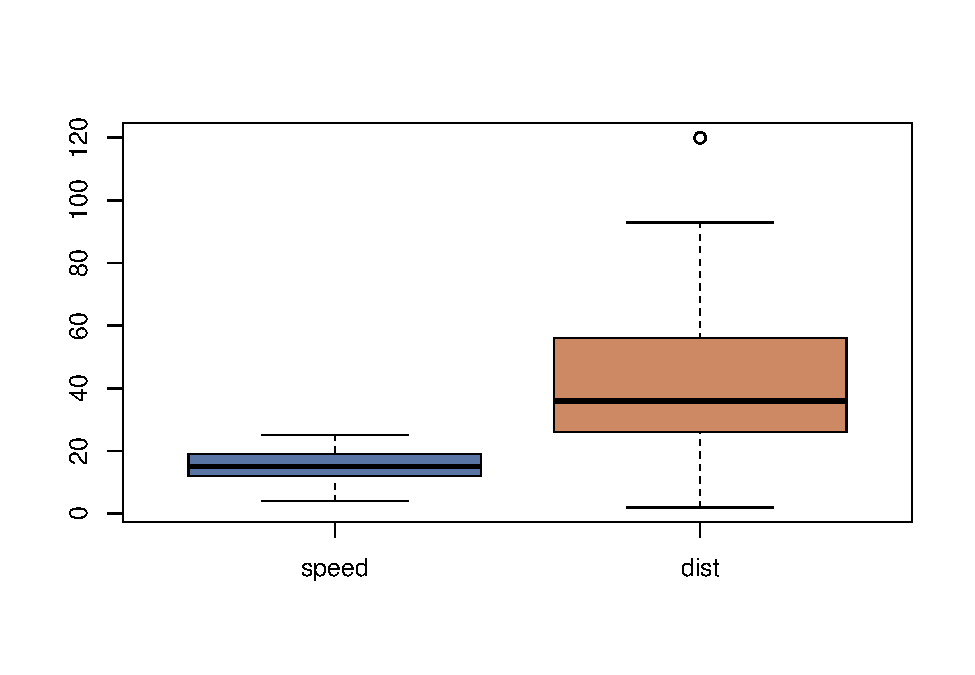
\includegraphics[width=7cm]{scdon2-UPV-report-template_files/figure-latex/unnamed-chunk-3-1} 

}

\caption{Déjà mieux.}\label{fig:unnamed-chunk-3}
\end{figure}

\normalsize

où l'on a:

\begin{itemize}
\tightlist
\item
  utilisé la commande \LaTeX~\texttt{\textbackslash{}tiny} pour changer
  la taille de la police (suivi de de
  \texttt{\textbackslash{}normalsize} pour revenir à la taille normale),
\item
  mis l'instruction \texttt{main\ =\ ...} sur la deuxième ligne,
\item
  utilisé \texttt{\textbackslash{}n} pour afficher le titre sur deux
  lignes.
\end{itemize}

\vspace{3em}

\textbf{Remarques} : Contrairement aux graphiques précédents, nous vous
demandons, pour effectuer les graphiques, d'utiliser le package
\texttt{ggplot2}. Voir
\url{https://juba.github.io/tidyverse/08-ggplot2.html} pour une courte
introduction.

\chapter{Inférence statistique et
modélisation}\label{infuxe9rence-statistique-et-moduxe9lisation}

Dans cette partie, vous pourrez utiliser les outils et méthodes vus au
semestre précédent pour analyser les liens entre les variables.

Pour cela, vous pourrez utiliser les tests du \(\chi^2\), test du
coefficient de corrélation linéaire, test d'Anova, la droite de
régression linéaire.

Vous pourrez également proposer des modèles pour faire du clustering
(k-means, CAH), de la classification (K plus proches voisins par
exemple) comme vu en Science des données 1.

\section{La droite de régression linéaire : un premier
exemple}\label{la-droite-de-ruxe9gression-linuxe9aire-un-premier-exemple}

Si on souhaite expliquer les variations d'une variables réponse \(Y\) en
fonction d'un certain nombre de prédicteurs \(x_1,\ldots,x_p\), on peut
utiliser un modèle de régression linéaire simple (\(p=1\)) ou multiple
(\(p>1\))

\[
Y_i = \beta_0 + \beta_1 x_{1i} + \cdots +\beta_p x_{pi} + \epsilon_i, \qquad i=1,\ldots,n.
\] où l'on présuppose que les \(\epsilon_i\) sont i.i.d.~\(N(0,1)\) pour
tout \(i=1,\ldots,n\) (\(n\) étant la taille de l'échantillon).

Vous pourrez toujours consulter avec profit les Chapitre 11--13 du livre
sur R :

\url{http://biostatisticien.eu/springeR/livreR.pdf}

Ces chapitres détaillent l'utilisation de certains tests et modèles sous
\texttt{R}.

\chapter{Discussion}\label{discussion}

Placer les résultats que vous avez obtenus dans le chapitre précédent en
perspective par rapport au problème étudié.

\chapter{Conclusion et perspectives}\label{conclusion-et-perspectives}

Quelles sont les conclusions principales? Quelles sont vos
recommandations pour le commanditaire? Quelles analyses subséquentes
pourraient être faites dans le futur?

\bigskip

On attend de vous deux types de perspectives : des perspectives à court
terme pour améliorer rapidement votre approche et des perspectives à
plus long terme qu'elles soient liées à la science des données ou au
domaine métier pour lequel vous avez travaillé.

\bigskip

Lister également les difficultés rencontrées dans la partie BD (e.g.,
taille de la base, manque de données, \ldots) et dans la partie
statistique.

\chapter*{Bibliographie}\label{bibliographie}
\addcontentsline{toc}{chapter}{Bibliographie}

\phantomsection\label{refs}

\bibliographystyle{elsarticle-harv}
\bibliography{references}

\chapter*{Annexes}\label{annexes}
\addcontentsline{toc}{chapter}{Annexes}

Il faut utiliser les annexes de façon judicieuse. C'est ici que l'on
place des résultats trop volumineux pour apparaître dans le corps du
rapport. Ou bien des résultats (e.g., graphiques) moins intéressants que
les autres. Cela permet de limiter le nombre de pages du coeur du
rapport, et d'ajouter des détails dans cette partie pour le lecteur
désireux d'en savoir plus.

\section*{\texorpdfstring{\textbf{Codes}}{Codes}}\label{codes}
\addcontentsline{toc}{section}{\textbf{Codes}}

Ajouter vos codes informatique ici. Les codes doivent être correctement
indentés et commentés.

\section*{\texorpdfstring{\textbf{Tables}}{Tables}}\label{tables}
\addcontentsline{toc}{section}{\textbf{Tables}}

Si vous avez des tableaux supplémentaires, vous pouvez les ajouter ici.

Utiliser \url{https://www.tablesgenerator.com/markdown_tables} pour
créer des tables Markdown simples, ou bien utiliser \LaTeX.

\begin{enumerate}
\def\labelenumi{\arabic{enumi}.}
\tightlist
\item
  Table Markdown
\end{enumerate}

\begin{longtable}[]{@{}lcr@{}}
\caption{une légende au-dessus du tableau.
\label{tab7.1}}\tabularnewline
\toprule\noalign{}
Les tables & sont & cool \\
\midrule\noalign{}
\endfirsthead
\toprule\noalign{}
Les tables & sont & cool \\
\midrule\noalign{}
\endhead
\bottomrule\noalign{}
\endlastfoot
col 1 est & alignée à gauche & \$1600 \\
col 2 est & centrée & \$12 \\
col 3 est & alignée à droite & \$1 \\
\end{longtable}

Aligner les nombres de la troisième colonne sur la droite permet
d'afficher les unités au-dessus des unités, les dizaines au-dessus des
dizaines, etc. Il faut toujours privilégier cette présentation.

\vspace{3em}

\begin{enumerate}
\def\labelenumi{\arabic{enumi}.}
\setcounter{enumi}{1}
\tightlist
\item
  Table Latex
\end{enumerate}

\begin{table}[h]
\centering
\caption{une légende au-dessus du tableau}
\label{tab7.1}
\begin{tabular}{lcr}
\hline
Les tables & sont & cool \\
\hline
col 1 est & alignée à gauche & 1600 \\
col 2 est & centrée & 12 \\
col 3 est & alignée à droite & 1 \\
\hline
\end{tabular}
\end{table}

\textbf{Remarques}

\begin{itemize}
  \item \{lcr\} : gauche (l), centré (c), droite (r)
  \item \verb|\caption| place la légende au-dessus
  \item \verb|\label| permet de référencer le tableau (\verb|\ref{tab7.1}|)
  \item Les nombres sont bien alignés à droite dans la 3\ieme{} colonne
\end{itemize}







\end{document}

